%!TEX root = /Users/markelikalderon/Documents/Git/timaeus/timaeus.tex
\chapter{Embodiment} % (fold)
\label{cha:incarnation}

\section{Cosmic and Encosmic Embodiment} % (fold)
\label{sec:cosmic_and_encosmic_incarnation}

There are similarities between cosmic and encosmic embodiment. The generation of the body of the Cosmos and its ensoulment and the generation of the human body and its ensoulment are in many ways similar, but there are important differences. 

First, there is a difference in agency. Whereas the Demiurge generates the body of the Cosmos and the soul that animates it, the Young Gods, generated by the Demiurge, act on His behest in generating the human body. At least the immortal part of the soul is generated by the Demiurge with similar materials, if less pure, than the materials from which the World Soul was generated. The difference in agency is explained by the limitations of the Young Gods' power of generation. In generating mortal beings, the Young Gods imitate Demiurgic activity. Their imitation is imperfect, however. Whereas the Demiurge generates immortals, the Young Gods generate only mortals. This is precisely why they are assigned this task. In order for a sensible living being to be truly comprehensive, it must contain within itself all manner of mortal living beings, and the Cosmos is a comprehensive sensible living being in order to better resemble the Paradigm, a comprehensive intelligible living being. 

Second, there is a difference in body. The bodies of mortal beings are importantly different from the body of the Cosmos that contains them. Mortal beings contained within the Cosmos are embedded in an environment with strong powers. The Cosmos, by contrast, is not embedded in an environment. There is nothing beyond the limits of the Cosmos, neither strong powers, nor space, nor void. Mortal beings depend upon and must defend against strong powers in their environment. Consequently, they themselves have a number of powers that are only ever exercised in an environment. That mortal beings are equipped with the instruments of these powers explains the way their bodies differ from the body of the Cosmos. 
% Specifically, the bodies of mortal beings differ in morphology from the body of the Cosmos, and that they are endowed with the instruments of environmental powers explains this difference.

Third, there is a difference in soul. The human soul has mortal and immortal parts. While the Young Gods generate the mortal part of the soul, the Demiurge generates the immortal part from the same material, if less pure, that He used to generate the World Soul. Like the World Soul, it is composed of the Circles of the Same and the Different, and though Timaeus does not say so explicitly, presumably the immortal part of the human soul is structured in the same way with proportional divisions. However, whereas the motions of the World Soul are unwaverable, the motions of the immortal part of the human soul are waverable---they may be affected by strong powers in the sensible environment. Moreover, unlike the Cosmos, human beings have, in addition, mortal parts of the soul. The mortal parts of the soul confer on the living being powers only ever exercised in an environment. That mortal beings are embedded in an environment with strong powers thus explains why their souls have mortal parts and why the motions of their soul may waver. The souls of mortal beings have a mortal part to endow them with environmental powers.

Fourth, soul and body are differently related. The World Soul encompasses the body of the Cosmos. Though some commentators may try to resist it, Timaeus spatial language is clear. The body of the Cosmos is contained within the World Soul. The immortal part of the human soul, by contrast, is encompassed by the human body. The immortal part of the soul is contained within the human body. It is bound to the marrow that composes the brain which is encased in the skull which is itself covered by flesh and hair. Just as the skin and hair protect the skull, the skull itself protects the brain and so preserves its bond with the immortal part of the soul. In this way, the body is organized so as to protect its bond with the immortal soul that it contains and that animates it. Mortal beings are embedded within the immortal Cosmos in the way that the Cosmos is not. That mortal living beings are embedded in an environment with strong powers explains how their soul and body are differently related.

Fifth, there is a difference in narrative order. Timaeus narrates the generation of the body of the Cosmos before narrating how it became ensouled. This narrative is reversed when it comes to the generation of human beings. Timaeus narrates the embodiment of the human soul before narrating the generation of the human body. This narrative reversal is accompanied by a perspectival shift. Timaeus narrates the incarnation of the human soul from the perspective of the human soul, the dramatic highpoint of which is Timaeus vivid description of the shock of embodiment. The ensoulment of the body of the Cosmos (34a8--34b10) and the embodiment of the World Soul (36d8--e5), by contrast, are impersonally presented. This perspectival shift is ethically significant. In dramatizing the shock of embodiment undergone by a newly incarnate soul, Timaeus makes vivid the ethical challenges faced and the need for salvation, thus laying the groundwork for his sensory soteriology (chapter~\ref{cha:the_end_of_vision_and_audition}).

The present chapter will follow the order in which Timaeus narrates the embodiment of the human soul and the generation of the human body. The differences highlighted above shall be further explained and their significance assessed (all but one---the mortal soul shall be discussed in chapter~\ref{cha:the_flesh_and_the_mortal_soul}). Just as the Cosmos lacks certain features since it lacks an environment, mortal beings have certain features since they are embodied and embedded in an environment with strong powers that they depend upon and must defend against. Again, the principle lesson for the philosophy of perception shall be the environmental nature of perception. Sensory powers are only ever exercised on aspects of the sensible environment in which the embodied percipient is embedded.

% section cosmic_and_encosmic_incarnation (end)

\section{The Demiurge's Address} % (fold)
\label{sec:the_demiurge_addressing_the_gods}

The Demiurge addresses two classes of gods. Specifically, the Demiurge addresses, on the one hand, the gods that manifestly revolve. These are visible gods. They are the celestial bodies such as the fixed stars. The Demiurge addresses, on the other hand, the gods that are not simply visibly manifest but manifest themselves at will. These are the Titanic and Olympian gods familiar from the poets and state religion including Athena---perhaps, significant given that Timaeus' speech is delivered on the occasion of Her festival. The Young Gods are rational co-participants of Demiurgic activity, and the Demiurge, in His address, reveals to them both His intentions, and the reason for their involvement in carrying out His intentions.

The address itself divides into three parts:
\begin{enumerate}[(1)]
	\item A discussion on the nature of bonds forms the basis of the assurance that the Demiurge gives the Young Gods. Though not wholly immortal, they need not fear death, since only what is evil would undo the bonds of what is well-fitted and good.
	\item The Demiurge instructs the Young Gods to generate the three remaining kinds of mortal beings. This they must do, since the Demiurge can only generate immortal beings, and mortal beings are required to complete the Cosmos conceived as a comprehensive sensible living being.
	\item The Demiurge explains that his role in the generation of mortal beings will be limited to generating the immortal part and instructs the Young Gods to weave what is mortal into what is immortal.
\end{enumerate}


(1) The Demiurge's discussion of bonds has an antecedent in Timaeus' speech, specifically in the proportionate bonds that unite the opposed extremes of fire and earth in amity in the body of the Cosmos. The Young Gods, like the body of the Cosmos, are compounded. And what unites the constituents of the compound into a whole are bonds. Though the Demiurge does not say, presumably these are proportionate bonds (compare 69b). After all, the fairest bond that most perfectly unites what it joins is proportion (\emph{analogia}, 31c2--4). 

What are united by the bonds that generate the Young Gods? \citet[]{Taylor:1928qb} posits two models. What is united by bonds is either, first, the materials that are combined in the generation of their soul or, second, what is united by bonds is their soul and body. Timaeus does not explicitly opt for one or the other of these models.

The first thing that the Demiurge does is explicitly state a principle that may be cause for concern, at least for any young god that may fear death. (If they are, indeed, capable of fear. This may be less an element of divine psychology than a convenient dramatic device.) All that are joined together by bonds may be undone. This is the reason that the Young Gods are not wholly immortal and indissoluble. Corresponding to Taylor's two models for what are united by the bonds that generate the Young Gods are two models of their death. Death is an undoing of what has been bound in generation, and since the two models differ in what has been bound in generation, they yield different models of death. On the first model, the undoing of the Young Gods is the dissolution of their soul into the constituents that entered into their mixture. Soul, recall, is generated from a mixture of indivisible and divisible Being, Sameness, and Difference. Should the Demiurge undo the soul of a young god, the one would dissolve again into the many. On the second model, the undoing of the Young Gods is the dissolution of their soul-body union, the separation of the soul from the body that it animates. On the second model, the separation of the soul from the body that it animates is straightforwardly a kind of death since the soul, in being separated, no longer animates the body. What was once living is now dead. 

The Young Gods are not wholly immortal. The qualifier ``wholly'' already hints at Demiurgic assurance. After all, not being wholly immortal is consistent with being partly or even potentially immortal. His assurance consists in the claim that only what is evil would undo the bonds of what is well-fitted and good. That principle only constitutes an assurance against the background of three further assumptions. 

First, it is assumed that the Young Gods are well-fitted and good. For if they are not, the principle does not say that it would be evil to undo that which is ill-fitted and bad, and so no assurance would be given. 

Second, it is assumed that the Demiurge, as the maker of these bonds, is not evil. For if He were evil, He would lack the motive to preserve what is well-fitted and good. But the Demiurge is benevolent and ungrudging. He is overflowing with goodness and not at all evil. 

Third, there is a further asumption here, namely, that only the Demiurge has the power to undo the bonds by which the Young Gods were compounded. For suppose this power was not the Demiurge's alone. Then some other agent could be the cause of their undoing. Even if the Demiurge, being benevolent and ungrudging, shall not undo the bonds that join them, some other agent may yet exercise this power should they be suitably evil. This last assumption was earlier made explicit in Timaeus discussion of the elemental composition of the body of the Cosmos (32c3--5) and will be made explicit again in the discussion of the shock of embodiment (43d) and in Timaeus' warning that it is impious to empirically investigate color mixture---only God is wise enough and powerful enough to blend the many into one and dissolve the one into many (68c7–d7).

The Demiurge ends this portion of His address with a hyperbolic claim that should be understood as the expression of His overflowing goodness. The Demiurge is benevolent and ungrudging and would not will the undoing of what is well-fitted and good. The Demiurge now represents His will has a greater bond than what bound them in generation. By Timaeus' lights at least, this Demiurgic claim is hyperbolic. Again, he has explicitly stated that the fairest bond that most perfectly unites what it joins is proportion (\emph{anologia}, 31c2--4). If the Demiruge's will is greater still, does that not mean that the bond that it constitutes is fairer and more perfectly unites what it joins? If so, the Timaean principle is false. The hyperbole is not a false boast, nor meant to mislead, but rather dramatizes the benevolent and ungrudging nature of the Demiurge whose overflowing goodness is the real guarantee of the immortality of the Young Gods. 

(2) In the second part of His address, the Demiurge instructs the Young Gods to generate the three remaining kinds of mortal beings. The Demiurge does not simply command them to do so, but explains why He needs them to fulfill His intentions. The Young Gods are rational co-participants in Demiurgic activity. In order for the Cosmos to be a comprehensive sensible living being and so contain within it every kind of sensible living being, mortal beings must be generated, and this requires rational cooperation.

According to Timaeus, the Demiurge intends for the Cosmos to contain four kinds of sensible living beings (39e11--40a2):
\begin{enumerate}[(a)]
	\item the Heavenly gods, celestial bodies such as the fixed stars
	\item the winged beings that traverse the air
	\item the beings that inhabit the water
	\item the beings that go by foot on earth
\end{enumerate}
Each kind of sensible living being is associated with a kind of primary body. The Heavenly gods are composed of fire---for the most part. This could mean a number of things. On the first alternative, the Heavenly god are composed of fire and other primary bodies with fire predominating. On the second, while some Heavenly gods are composed of fire, others are not. On the second alternative, the Heavenly gods composed of fire are presumably the fixed stars and the Sun, while those that are not are presumably wanderers such as the Moon. On the third, hybrid, alternative, the Heavenly gods are all predominately composed of fire, it is just that some, such as the fixed stars and the sun, are composed of a greater proportion of fire and are consequently brighter. I am inclined to accept the third alternative. 

Like the first alternative, the third maintains that all the Heavenly gods are composed predominantly of fire. Indeed, the Heavenly gods live in the region of the Cosmos where fire naturally accumulates. Immediately below that region, in the region of the air, is where winged creatures fly. There are living beings that inhabit the water such as fish that swim in the sea. Finally there are living beings that walk upon the Earth. (At least typically, Timaeus acknowledges living beings, such as serpents and worms, that lack feet to walk with and yet wiggle upon the Earth, 92a.) So each kind of sensible living being is associated with a kind primary body and lives in the region of the Cosmos where, thanks to the winnowing motion of the Receptacle, the associated primary body naturally accumulates. Whereas the Heavenly gods are immortal, at least by Demiurgic assurance, the three remaining kinds of living being are mortal.

The Demiurge's reason is comprehensiveness. There should be four kinds of sensible living beings in order to correspond to the four kinds of intelligible living beings contained within the Paradigm. The Paradigm is an intelligible living being. Moreover, it is a comprehensive intelligible living being. It contains within itself all other intelligible living beings. But to be truly comprehensive and so better resemble the Living Being, the Cosmos must contain within itself every kind of sensible living being. So the comprehensiveness of the Cosmos is only perfected by the activity of the Young Gods, at behest of the Demiurge, in generating the three remaining kinds of mortal living beings.

Thus far in the narrative, the Demiurge has generated immortal beings. Indeed, given that his power is the expression of His overflowing goodness, He is only capable of generating immortals. But to be truly comprehensive, the Cosmos must contain within itself the three kinds of mortal living beings. It is for this reason that the Demiurge assigns this task to the Young Gods. The Young Gods shall do so by imitating Demiurgic activity. However, the imitation is imperfect. While the Young Gods are capable of generating living beings, these will be mortal. The irony here should be evident. Imperfect mimetic activity is required to complete and so perfect the Cosmos.

That the Young Gods are immortal if not wholly immortal introduces a complication, since it reveals two dimensions along which the mimetic activity may be imperfect. That the Young Gods are not wholly immortal means that their immortality is predicated, in part, on the benevolence of the Demiurge. Does the mimetic imperfection of the Young Gods in generating mortal living beings consist in a failure of benevolence? That seems unlikely. Notice that in the case of the Young Gods, their bonds are potentially dissolved by the One who bound them. By contrast, the bonds by which mortal beings are generated dissolve not only by the agency of those who bound them. Strong powers in the sensible environment can dissolve these bonds, and not just the Young Gods that bound them. The mimetic activity of the Young Gods is imperfect in that they are not the sole agent of the dissolution of the bonds by which mortal beings are generated.

(3) Mortal beings shall have a part that deserves to be called ``immortal''. This part the Demiurge Himself shall generate. And with respect to the human soul, the Demiurge shall generate it in a way that parallels his generation of the World Soul. The human soul too shall be a mixture, though less pure, of indivisible and divisible Being, Sameness, and Difference. Moreover, it too shall be proportionally divided and fashioned into the Circles of the Same and the Different. The Young Gods task is to generate the specifically mortal parts of these living beings, borrowing corporeal material from the body of the Cosmos itself to which it shall return in full once the mortal being perishes. (Given that the divinity of the Cosmos, Feeble can thus be read as speaking on behalf of Timaeus when, in \emph{Henry IV Part 2}, Act 3, Scene 2, he proclaims that ``We owe God a death''.) Moreover, the Demiurge instructs the Young Gods to weave the mortal parts into the immmortal parts. So the Young Gods task is not only to generate the mortal parts of sensible living beings but to join these through weaving to the immortal parts that the Demiurge Himself generated.

Completing and so perfecting the Cosmos is thus not a task that the Demiurge simply leaves to the Young Gods. Since even mortal living beings have immortal parts, and these can only be generated by the Demiurge, the completion and perfection of the Cosmos is a coordinated activity of the Demiurge and the Young Gods acting on His behest. And as this coordinated activity is rational, the Demiurge has explained not only his intentions but the reasons for the involvement of the Young Gods in fulfilling them.

The metaphor of weaving the mortal parts into the immortal parts is worth pausing over. (On ancient weaving and the Greek standing loom in particular see \citealt{Burke:2010aa,Crowfoot:1936aa,Flores:2006aa,Hoffmann:1964aa}.) It was used as well to describe how the soul of the Cosmos and its body were fitted together (36d8–e5). Indeed, Plato frequently refers to weaving. References to weaving can be found in the \emph{Theaetetus} (202b3), the \emph{Sophist} (259e6, 262d4), the \emph{Statesman} (279a--283a), and \emph{Cratylus} (387e--390b). Indeed, the \emph{Statesman} (279a--283a) and Aristophanes' \emph{Lysistrata} (565--87) are our main textual sources concerning weaving in antiquity (on weaving in the \emph{Statesman} see \citealt{Cole:1991qq}). So frequent and so vivd are Plato's references to weaving that \citet[44, n1]{Skemp:1952aa} reports that a replica of an ancient loom was constructed on this basis in consultation with a modern weaver. It is perhaps worth recalling an aspect of the circumstance of Timaeus's speech. The occasion is the Panathenaic festival, which explains the presence of such notable non-Athenians as Hermocrates, the Syracusan general, and Timaeus, who hailed from Locri in southern Italy. The festival is dedicated to Athena, goddess of weaving. Weaving requires intelligence, which is why it is associated with Athena. The festival involved weaving a \emph{peplos} for the sculpture of Athena in the Acropolis. This figured prominently in the festival's procession. At one point, the \emph{peplos} featured as the sail of a ship that was part of the Panathenaic procession (Scholia on Homer, \emph{Illiad} 5 734). According to Philostratus: 
\begin{quote}
	The robe of Athene that was hung on the ship was more charming than any painting, with folds that swelled before the breeze, and the ship, as it took its course, was not hauled by animals, but slid forward by means of underground machinery. Setting sail at the Cerameicus with a thousand rowers, it arrived at the Eleusinium, and after circling it, passed by the Pelasgicum: and thus escorted came by the Pythium, to where it is now moored. (Philostratus, \emph{Vitae Sophistarum} 2 550; \citealt[147]{Wright:1922aa})
\end{quote}
So important was the contribution of the weavers (\emph{egastinai}) that they were portrayed in a section of the Parthenon frieze (see~\ref{fig:frieze}). Thus the occasion of Timaeus's speech itself highlights the significance of weaving. 

\begin{figure}[htbp]
     \centering
         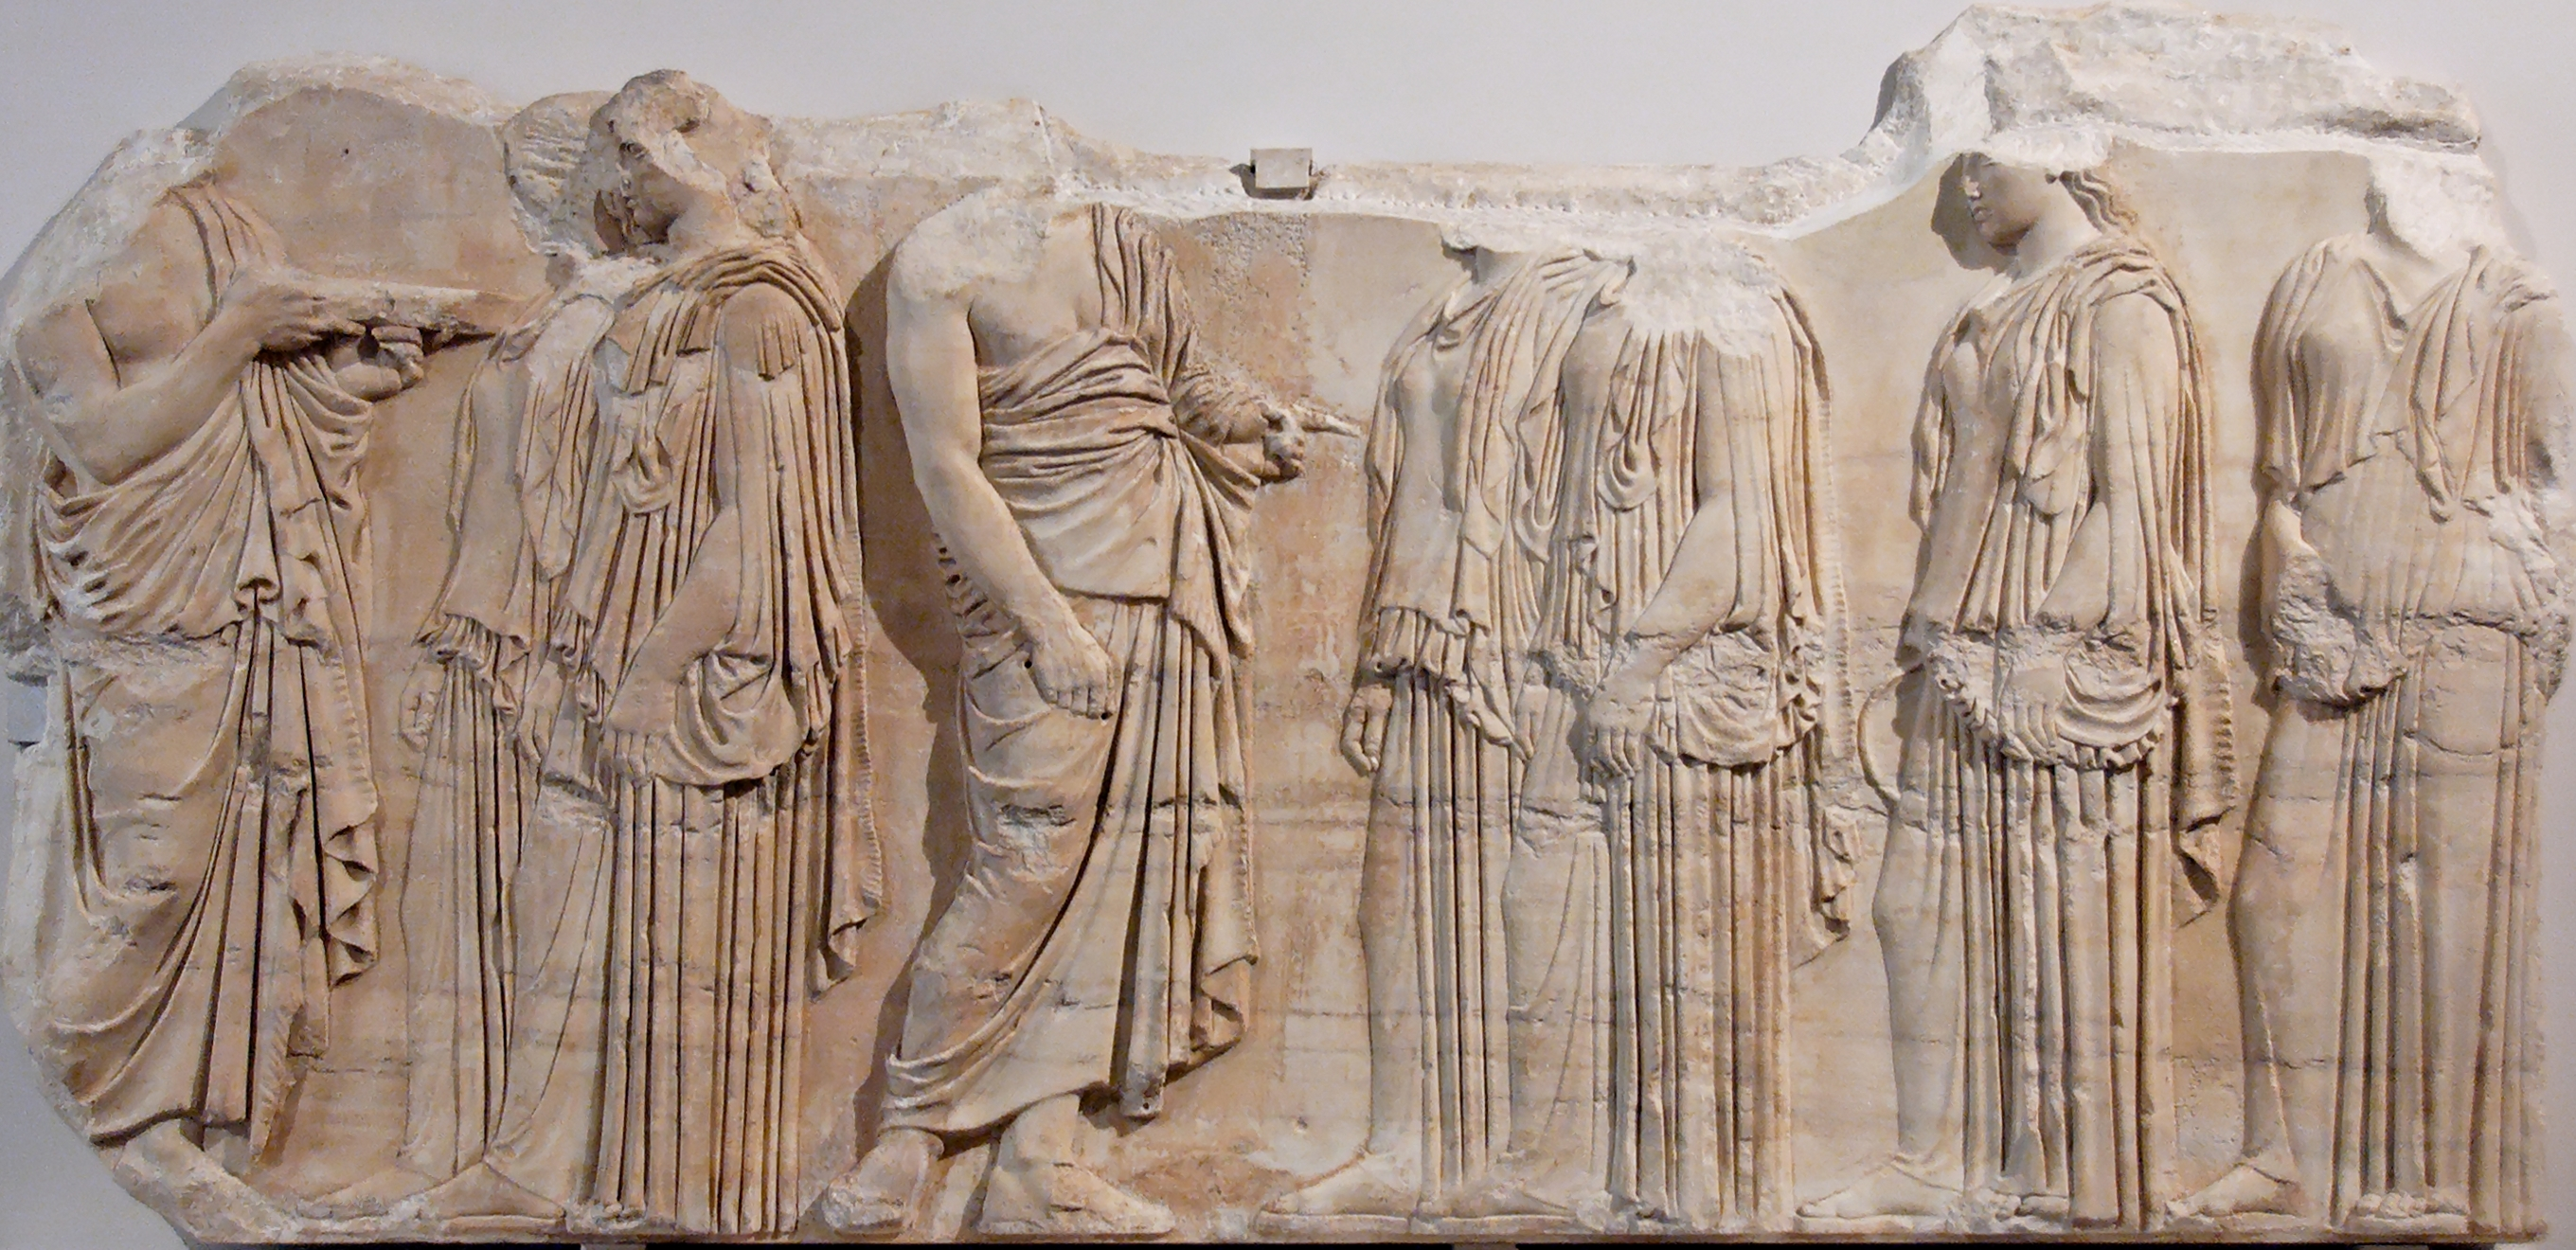
\includegraphics[scale=1.4]{graphics/egastinai_frieze.jpg}
     \caption{\emph{Egastanai} frieze, East VII, 49--56, ca 445--435 BCE Louvre}
     \label{fig:frieze}
\end{figure}

Since weaving requires intelligence, the Young Gods' weaving mortal onto the immortal is a rational activity. In acting on the Demiurge's behest the Young Gods are not instruments of the Demiurge's activity. They are not the instruments by which the soul is united with the body the way that a shuttle, say, is an instrument of weaving. The Young Gods are agents of that activity. Engaging in such activity requires intelligence and so it is a rational activity. The Young Gods act on behest of the Demiurge, not by being the instruments of Demiurge's activity, but by being rational co-participants in Demiurgic activity, the completion of a comprehensive sensible living being. 

There are two components to weaving thread or yarn into fabric. There is the warp (\emph{stēmōn}) and the weft (\emph{krokē}). The warp are vertically arrayed thread or yarn. These are stationary and held in tension in the loom as the weft, horizontally arrayed thread or yarn, are drawn through. The thread or yarn that compose the warp are typically thicker or sturdier then the thread or yarn that compose the weft since they supply structural support for the weft. The Greeks used standing looms, where the warp hung from a horizontal bar and were held in tension by attached clay weights (\emph{agnuthes} or \emph{laiai}) (see Figure~\ref{fig:loom}). Alternate warp threads were attached to one of two horizontal bars (\emph{kalamos} and \emph{kanōn}) which were used to create the ``shed'', the space between the alternating warp threads through which the shuttle (\emph{kerkis}) carrying the weft thread would pass. The weft thread was then beaten upward in place with a wooden spatula (\emph{spathē}). 

As Herodotus reports, beating the weft upward contrasts with the Egyptian method, ``Other nations weave by beating the weft upward, the Egyptians downward'' (\emph{Historia} 2.35.10). There is an irony here. Herodotus' description occurs in a passage describing how the Egyptian customs are the reverse of the Greek. Herodotus' intent is to highlight the superiority of Greek culture. But with the advantage of gravity, the Egyptian method, in the end, predominated. (At least in the West, if not universally. While of Neolithic origin, \citealt[1--2]{Hoffmann:1964aa}, observed the continued use of standing looms among the Sami on an island off the coast of Norway.) An effect of this is that it is we who are now surprised at the Greek standing loom and the way that its use reverses the pre-industrial custom of beating the weft down. (Outside of specialist hand weavers and weaving enthusiasts, that custom is present in the West, if at all, only as a historical memory of a practice eclipsed by the industrial revolution.)

Perhaps the effort to beat the weft upward, against gravity, is meant to echo the effort, in the \emph{Phaedrus} myth, exerted by mortal souls to ascend to the rim of the Heavens in chariots pulled by two horses one of which is inclined to pull downward. If the rim of the Heavens is not only circular (it revolves) but spherical, and the downward inclination is toward its center where the Earth is located (see \citealt[114--5]{Dicks:1970aa}), then the \emph{Phaedrus} myth anticipates not only aspects of Timaeus' astronomy but his theory of direction as well. If beyond the periphery is nothing sensible and corporeal but, rather, the intelligible and incorporeal, then the myth not only contains astronomical commitments but moral ones as well. Only the virtuous complete the ascent and attend only to the intelligible. The vicious, by contrast, are dragged down by their concern for the sensible and the corporeal. The weft, is similarly inclined downwards by the force of gravity, toward the Earth and away from the circumference of the Heavens, and the mortal beings that result from the soul--body union are inclined to the sensible away from the intelligible because of the bodily component of the union represented by the weft. Moreover, this is an ethical challenge dramatized by the shock of embodiment (42e5--44d2, discussed in section~\ref{sec:the_shock_of_embodiment}) and providentially accommodated by the Young Gods providing, at the Demiurge's behest, eyes to see the Heavens with (46e6–c4, discussed in chapter~\ref{cha:the_end_of_vision_and_audition}). Observing the Heavens with rational attention counteracts the adverse effects of the sensible and the corporeal on the soul (since the linear motion of \emph{aisthēsis} has the tendency to distort the circular motion of the soul, see section~\ref{sec:the_shock_of_embodiment}).

\begin{figure}[htbp]
     \centering
         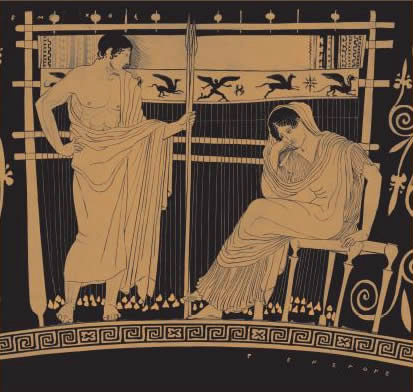
\includegraphics[scale=0.80]{graphics/penelope_chiusi.jpg}
     \caption{Penelope and Telemachos with loom, Attic red cup, side B, ca 440 BCE, Museo Nazionale, Chiusi}
     \label{fig:loom}
\end{figure}

If the bodily component of the soul--body union is the weft, then the immortal part of the soul is the warp. The fixed stationary character of the warp and the fact that it supports the weft makes it an apt metaphor for the immortal part of mortal living beings. According to Timaeus, the immortal part supports and governs the mortal part. Does this parallel or contrast with the way in which the soul of the Cosmos was interwoven with its body? Is the body of the Cosmos weft to the World Soul's warp? The structural support provided by warp would, again, be an apt image for how all that is corporeal is constructed within the World Soul (see chapter~\ref{sec:the_embodiment_of_the_world_soul}). However, Timaeus' language here, ``everywhere interwoven'' (\emph{pantē daiaplakeisa}), is not specific enough to support this interpretation all by itself. However, when read in light of the present passage, I find the interpretation both plausible and compelling.

% section the_demiurge_addressing_the_gods (end)

\section{The Immortal Part} % (fold)
\label{sec:the_immortal_part}

Having addressed the Young Gods, and explained his intentions and the reasons for his involvement of the Young Gods in completing and so perfecting the Cosmos, the Demiurge immediately turns to his own role in the generation of the three kinds of mortal beings. Specifically, the Demiurge sets about generating their immortal part. 

The immortal part of mortal beings is the soul, or at least the immortal part of the soul. This is generated in a parallel fashion to the generation of the World Soul. Indeed the Demiurge works with the same materials. The World Soul is a mixture of indivisible and divisible Being, Sameness, and Difference. The remains of these are now mixed in the same manner. The ``remains'' refer not to a residue of the previous mixture---that was all used up in the generation of the World Soul. I take it that the remains are the remaining ingredients of such a mixture, indivisible and divisible Being, Sameness and Difference (see \citealt[141 n10]{Archer-Hind:1888qd}, \citealt[255]{Taylor:1928qb}). Presumably, when Timaeus says that they are mixed in the same manner he means, among other things, that they are mixed in the same proportions. There is, however, a crucial difference, the present mixture lacks the uniform and invariable purity of the World Soul. As Timaeus elaborates for emphasis, it is of a second or third degree of purity. 

There is another notable difference whose significance is difficult to discern. Timae\-us describes an instrument of divine mixture, the \emph{kratēr}, not mentioned in his account of the generation of the World Soul. Though omitted in his description of its generation, the \emph{kratēr} must have been used to mix the World Soul since Timaeus describes the Demiurge as returning to the \emph{kratēr} to mix the soul of mortal beings. The Greek word \emph{kratēr} can mean the vase in which wine and water is mixed in proportions determined by the symposiarch, the master of the symposium (see Figure~\ref{fig:krater}). As such it is the visible symbol of the symposiarch's authority to determine the proportion of wine and water to be mixed and the rate at which the mixture is served. So understood it would be an apt image of the Demiurge's authority in determining the mixture of indivisible and divisible Being, Sameness, and Difference. 

\begin{figure}[htbp]
     \centering
         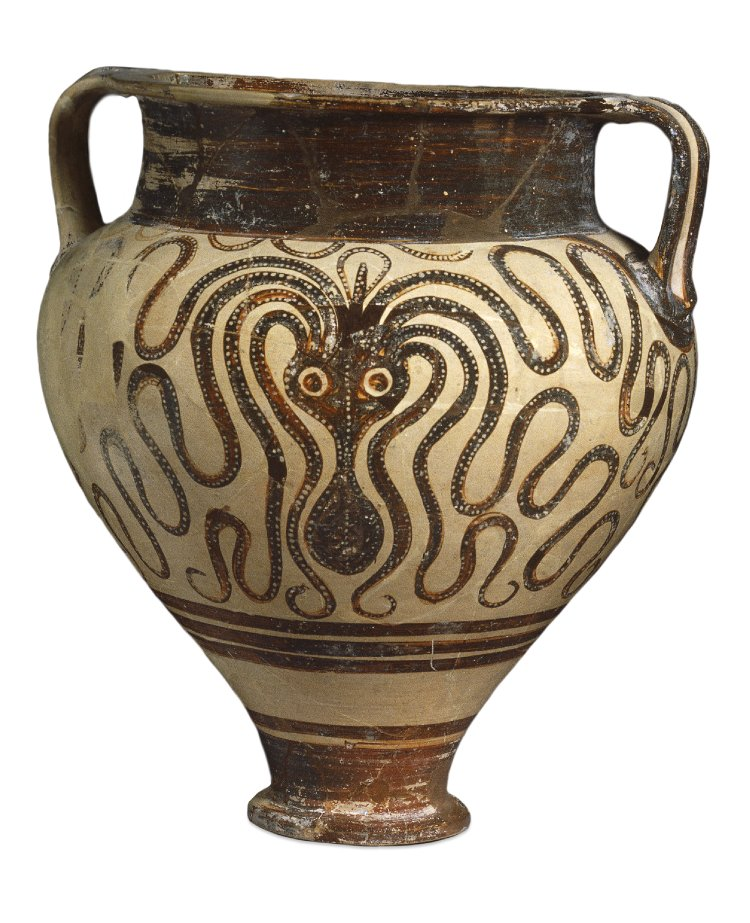
\includegraphics[scale=0.25]{graphics/krater.jpg}
     \caption{\emph{Kratēr} with octopus, ca 1375-1300BCE, British Museum}
     \label{fig:krater}
\end{figure}

There are other elements of the semantic field, however. The Greek word \emph{kratēr} can mean a volcanic crater which is typically bowl shaped. Though perhaps a less obviously apt meaning, the bowl shape of volcanic craters and their association with Hephaestus, god of metallurgy, can suggest another related sense which is, perhaps, more apt, namely, a crucible. An alloy, such as bronze, is a mixture of metals or metalloids which typically have properties distinct from its constituent ingredients. The effort involved in mixing Difference suggests the metallurgic production of an alloy in a crucible. The \emph{Chaldean Oracles} offers a different interpretation. The \emph{kratēr} is there represented as a divine womb (\citealt[]{Brisson:2003aa} and ). The womb metaphor is apt independently of the assignment of deity insofar as the \emph{kratēr} is the recipient of generative activity. One issue with the Chaldean interpretation is that, in a way, it is a return to an older model of generation that Timaeus can be seen as self-consciously replanting. Consider, for example, the role of sexual reproduction in Hesiod's \emph{Theogony}. Timaeus, by contrast, provides a model of cosmological explanation based, not on sexual reproduction, but on craftsmanship. The alternative senses need not be competing. Perhaps Timaeus intends the different associations of a range of these to apply, in some measure, to the Demiurgic \emph{kratēr}. (After all, we have already seen, chapter~\ref{sec:the_embodiment_of_the_world_soul}, Timaeus simultaneously pursuing distinct imagery in his account of the soul-body union.)

Another element of Timaeus' account that requires comment is the way in which the souls of mortal beings are generated from the same materials as the World Soul, if less pure. I am unsure what Timaeus so much as could mean by purity here. On the most straightforward understanding, the mixture would be pure if it consisted solely of indivisible and divisible Being, Sameness, and Difference. And it would be impure if it contained, in addition, some other material. But what other materials? Rest and Motion? It is hard to understand Timaeus' talk of purity in terms of the absence of the alien. So what could purity amount to here? Perhaps it is a matter of the exactness of proportion with which these materials are mixed (\citealt[141 n11]{Archer-Hind:1888qd} makes this suggestion, and Gábor Betegh made a similar suggestion to me in conversation). That would avoid the previous difficulty, but the problem is that balance and harmony are not purity, even in an extended sense of purity. Another idea concerns the degree of mixture. Perhaps the souls of mortal beings are incompletely mixed compared to the World Soul. Being incompletely mixed, the substance is not as homogenous as the substance of the World Soul. This suggestion suffers from the same problem as the previous one. Inhomogeneity is not impurity, even in an extended sense. Suppose, however, Timaeus did have in mind, among other things, the metallurgic production of an alloy in a crucible. Recall the properties of an alloy may not be shared with the properties of the materials from which it was mixed. The inhomogeneities induced by an incomplete mixture would mean that while some parts are a genuine alloy, others are not. Perhaps one might say that the alloy produced was impure due to such inhomogeneities. The present suggestion avoids the previous difficulties but lacks clear textual support. Overall it remains unclear what, precisely, talk of purity amounts to here.

While it is unclear what exactly Timaeus means by purity, the consequences of impurity are clear. The human soul is like the World Soul in its composition and mixture. They are generated from the same materials and mixed in the same proportions. The human soul is unlike the World Soul in being less pure, indeed to a second or third degree. The World Soul is thus prior not only in birth but in dignity. The generation of the World Soul is temporally prior to the generation of the human soul and so prior in birth. And the World Soul is generated from a purer mixture of the same materials from which the human soul is mixed and is thus prior in dignity, owing to its more perfect purity. The World Soul is very much the elder sibling of the human soul. Indeed, Plotinus describes them as sisters (\emph{Ennead} 2 9.18 14--17). 

Calcidius offers a related explanation for the impurity of the mixture from which the souls of mortal beings were generated and the consequent inferiority of their dignity. Such souls are destined to be embodied, and their impurity facilitates their union with the corporeal (\emph{In Timaeum} 140). While the World Soul is itself united with the body of the Cosmos, unlike mortal beings, it does not suffer an encosmic existence. The World Soul, when embodied, is not embedded in and environment and so is not subject violent affection from without. So Calcidius' explanation, if adequate, must be understood as facilitating, not embodiment, but encosmic embodiment, understood as embodied existence embedded in an environment with strong powers.

Not only is the human soul like the World Soul in its composition and mixture, they are also similarly constructed. Just as the Demiurge constructed the Circles of the Same and the Different from the pure mixture from which the World Soul was generated, the Demiurge constructs the Circles of the Same and the Different from the impure mixture from which the human soul was generated. Timaeus later confirms this in his narrative of the shock of embodiment. Presumably, the Demiurge apportions the soul mixture in the same proportional divisions in the human soul as he did in the World Soul (this is confirmed at 43d in Timaeus' account of the shock of embodiment), though given the impurity, perhaps less precisely. Presumably, as well, just as the revolutions of the Circles of the Same and the Different determine the kinetic and cognitive powers of the World Soul, the revolutions of the Circles of the Same and the Different determine the kinetic and cognitive powers of the human soul. The human soul is at least capable of operating in alignment with the World Soul. And it is capable of this since it is generated from the same materials, mixed in the same proportions, and constructed in the same fashion.

The Demiurge divides the mixture into a number of souls equal to the number of stars. The Demiurge then assigns each soul to its own star. Timaeus describes this as each soul being mounted in a vehicle (\emph{ochēma}), such as a carriage or perhaps a chariot as in \emph{Phaedrus} 247b. The souls are mounted there, in the stars, so that the Demiurge may address them, as He explains the nature of the Cosmos and the Laws of Destiny to them, prior to their embodiment. (Timaeus' talk of soul-vehicles, here, will become a rich vein of psychological speculation for the Neoplatonists, and the Western source for the occult doctrine of astral bodies, see \citealt[appendix 2]{Dodds:1963ul} and \citealt{Finamore:1985aa}.) The stars, here, are the fixed stars as opposed to the wanderers  (see \citealt[141--2 n13]{Archer-Hind:1888qd}, \citealt[255--6]{Taylor:1928qb}, \citealt[143]{Cornford:1935fk}). This is clear from the one-to-one correspondence between the souls and the stars. After all, there are more souls than wanderers.

It is important to recognize that the fixed stars have their own souls that animate their fiery bodies. The souls mounted in them as in a vehicle are distinct from the souls of the Heavenly gods. They neither animate the fiery bodies of their stellar vehicles, nor do they otherwise move them. Unlike the \emph{Phaedrus} myth, the souls of mortal beings are mounted in their stellar vehicles as passengers, not drivers. The divine celestial beings in which they are mounted are ensouled and so direct their own movement in harmony with the revolutions of the World Soul. The souls of mortal beings are thus not embodied, at least not completely. What is envisioned here is, rather, a derivative corporeal presence prior to their embodiment. It is only when they are embodied, in the final phase of celestial descent, do the souls of mortal beings animate their proper bodies and direct their movement.

Why should the soul of mortal beings, in their pre-embodied state, be assigned to a star and be mounted in it as in a vehicle? After all, there was nothing in which the World Soul was mounted before it encompassed the body of the Cosmos. If anything, it would be more apt to say that the body of the Cosmos is mounted in the World Soul as in a vehicle. Like a carriage, the body of the Cosmos is carried within it. The souls of mortal beings, unlike the World Soul, are encosmic. After all, the World Soul is the soul of the Cosmos, not the soul of a sensible living being contained within the Cosmos. Perhaps the souls of mortal beings can only exist within the Cosmos if they are embodied, however incompletely. The bodies of the stars, when functioning as vehicles for the souls mounted in them, become surrogate bodies of pre-embodied souls. In being assigned to the stars, the souls of mortal beings in their pre-embodied state nonetheless secure for themselves a derivative corporeal presence within the Cosmos. 

Some support for this is given in 44e where Timaeus describes the human body as a vehicle for the soul. In this context, vehicle is meant quite literally as a means of locomotion. Only sensible living beings contained within the Cosmos have space within which to move in the six irrational linear motions. Only they are embedded in an environment with strong powers and space to move in. Only they require a means of locomotion. In this way, they contrast with the Cosmos that contains them, for beyond its limits is neither space nor void in which to irrationally move. The power of locomotion is environmental. It can only ever be exercised in an environment that circumscribes its possessor. And again at 69c, Timaeus describes the Young Gods as giving to the human soul its body as a vehicle. Though, here, it is unclear whether vehicle is exclusively meant as a means of locomotion.

There are two things that vehicle can mean. On the one hand, it may be a means of locomotion, such as a carriage or chariot, or it may be a bearer. Consider: a vehicle of expression is not a means of locomotion. It may bear what is expressed but it transports it nowhere, at least not literally. Though distinct, these meanings overlap. A means of locomotion may bear what it transports. But a bearer need not transport what it bears. Even in cases where these senses overlap, the conversational focus may be on one or the other. When the Demiurge mounts the pre-embodied souls in the stars as in vehicles, the souls travel along with the Heavenly revolutions. So their stellar vehicles are a mode of transport. But what is important is their presence within the Cosmos. It is only a corporeal presence within the Cosmos that secures for them a view on its contents and so puts them in an apt position for the Demiurgic address. And a corporeal presence requires a bodily vehicle understood as a bearer rather than a mode of transport, even if it is also a means of locomotion.

That souls can only exist within the Cosmos if they are embodied (perhaps derivatively, like the souls mounted in their stellar vehicles) potentially bears on the interpretation of the Timaean principle that intellect can only exist in soul, and soul in body. Specifically, it raises the possibility of a restricted reading of that principle. Soul must exist in body only if it exists within the Cosmos. The suggestion is that the principle is restricted to encosmic living beings. So understood, it is consistent with there being intellect without soul, and soul without body. It is just that these would lack a corporeal presence and so could not suffer an encosmic existence. 

Encosmic living beings exist in an environment that circumscribes them, the Cosmos. And in order to exist within that environment, encosmic living beings must be embodied. Timaeus thus postulates a link between embodiment and embeddedness. One must be embodied to be embedded in an environment. Embodiment may be insufficient for being embedded within in environment, however. The Cosmos is embodied but lacks and environment. But embodiment is necessary for being embedded within an environment. Corporeal presence is required for encosmic existence.

The Demiurge, in assigning each soul to its own star, affords them a Heavenly perspective on the Cosmos, an apt vantage point from which to be instructed as to the nature of the Cosmos and its foreordained laws. They need to be present in the Cosmos in order to have a view on it. In order to be present in the Cosmos, they need a corporeal vehicle, even a derivative one. And in order to have an apt vantage point on the contents of the Cosmos, they are mounted in the stars as in vehicles. And presumably, from their stellar vehicles, the perspective of each is directed toward the center of the Cosmos. After all, it is implausible to suppose that they are suffering from a cramped perspective of the inner circumference of the Cosmos. Moreover, the fixed stars have forward motion as they revolve along with the Circle of the Same in the World Soul. Their passengers thus enjoy a revolving view of the whole of the Cosmos. Having a view on the whole of the Cosmos, insofar as that is possible, is an apt vantage point from which to receive, from the Demiurge, an account of the nature of the Cosmos and the Laws of Destiny. 

The Cosmos is the subject of the Demiurge's address. Understanding that address involves thinking about the Cosmos, its subject. Recall the Eleatic pun (chapter~\ref{sec:the_cognitive_significance_of_circular_motion}). Thinking about (\emph{peri}) the Cosmos involves the soul's motion, understood as an incorporeal activity, around or about (\emph{peri}) the Cosmos. So perhaps the souls of mortal beings traveling around the Cosmos in their stellar vehicles is an image of their cognitive activity. In this way their locomotion, an irrational linear motion, would be harmonized with their thought, a rational circular motion (in the activity sense, see chapter~\ref{sec:the_cognitive_significance_of_circular_motion}).


% section the_immortal_part (end)

% section section_name (end)
\section{The Laws of Destiny} % (fold)
\label{sec:the_laws_of_destiny}

The Demiurgic address, where He explains the nature of the Cosmos and the Laws of Destiny to the souls of mortal beings, is bookended by two phases of a celestial descent. We have already described the first phase of celestial descent, the Demiurge assigning each soul to a star. This a descent insofar as the souls of mortal beings move from a hypercosmic to an encosmic existence. Notice that the \emph{kratēr} in which the souls were mixed is no part of the Cosmos. So when initially generated, the souls have only a hypercosmic existence. They only first appear in the Cosmos when they are mounted in their stars as in vehicles. After the address, prior to being embodied, the souls will be reassigned to the wanderers. So initially, they are assigned to the fixed stars moving along with the Circle of the Same in the World Soul. Subsequently, they are reassigned to the wanders moving along with the divided Circle of the Different. This reassignment is a descent in a different, more literal, sense. The fixed stars are at the circumference of the Cosmos, and the wanderers are between the circumference of the Cosmos and its center. And according to Timaeus' account of direction (62d4–10), movement from the circumference of the Cosmos toward its center is downward. The descent ultimately culminates in the soul's embodiment on Earth located at the center of the Cosmos. In the initial phase of the celestial descent, the assignment is one-one, in the subsequent phase, the assignment is one-many. The Moon, for example, will be assigned many souls. In the final phase of descent, in the shock of embodiment, each soul is assigned its own body to animate and the assignment is again one-one.

The soul's descent is not due to some fault, the sin of pride, say. Rather, the soul must descend to complete and so perfect the Cosmos. The Cosmos is only complete when it is comprehensive. Only if it is a comprehensive sensible living being can the Cosmos best resemble the comprehensive intelligible Living Being. The Cosmos is a sensible living being, but to be a comprehensive sensible living being, it must contain with in itself every other form of sensible living being. The Cosmos can only be a comprehensive living being if the souls of mortal beings descend. The soul must descend to complete and so perfect the Cosmos. In our cultural context, it is very easy to misread the soul's descent in terms of the Lapsarian Myth. And the moving and dramatic narrative of the shock of embodiment may encourage the thought that embodiment is retribution for some terrible sin. But that is Pauline theology. In Timaean theology, the soul's descent is an act of perfection not retribution.

There is a literary difference, whose significance I am unsure of, between Timaeus' presentation of the Demiurgic address to the Young Gods and his presentation of the Demiurgic address to the pre-embodied human souls. Whereas the former is presented in direct discourse, the latter is presented in indirect discourse (as Proclus observed, \emph{In Timaeum} 3 271-2, \citealt{Diehl:1903re}). Moreover the former is more specific and detailed than the latter. Perhaps Timaeus, or Plato in his guise, did not want to unduly interfere with the \emph{anamnesis} of the audience, and by extension, the reader.

The Demiurge in His address to the pre-embodied souls of mortal beings mounted in their stellar vehicles explains two things: (1) the nature of the Cosmos and (2) the Laws of Destiny. Timaeus, however, only reports the latter (presumably since the nature of the Cosmos is the subject of his entire discourse):
\begin{enumerate}[(1)]
	\item That the first birth is one and the same for all (41e3--5)
	\item That those who are sown in the instruments of time should grow to be the most god-fearing of living beings (41e5--42a1)
	\item That human nature is two-fold, the superior sex being called ``man'' (42a1--3)
	\item That \emph{aisthēsis} is native and common to all and the result of violent affection (42a3--7)
	\item That they shall be subject to desire (\emph{erōs}) mingled with pain and pleasure (42a7--8)
	\item That they shall be subject to fear and anger and all other emotions (42a8--b2)
	\item That those that master these shall live justly, and those that do not shall live unjustly (42b2--3)
	\item That those that have lived justly shall return again to their appointed star (42b3--6)
	\item That those that have lived unjustly shall be born as a woman in their second birth (42b6--7)
	\item That those who persist in living unjustly after their second birth shall be reborn in some bestial form that reflects their character (42b7--d3)
\end{enumerate}
The Laws of Destiny fall naturally into three parts. The first part, (1--3), sets out some general facts. The second part, (4--6), has a more explicit focus. In virtue of Necessity, the souls being addressed will be embodied, and the Demiurge explains some of the consequences of this to them. The third part, (7--10), concerns the ethical significance of embodied existence and the consequences of living justly or unjustly. The third part lays the groundwork for Timaeus' sensory soteriology discussed in the next chapter. The Demiurge is explicit about the motive of His address, to be blameless for any evil that follows from their actions once embodied. Everyone knows the score, and everyone has an equal shot, so no one should blame the Demiurge for being reincarnated in bestial form. Timaeus, here, clearly echoes the Socratic thought that the souls of mortal beings are the sole source of evil. From that thought he elaborates a theodicy of sorts. Let us briefly review these.

(1) \emph{That the first birth is one and the same for all (41e3--5).} That the Demiurge calls it the ``first'' birth manifests Timaeus' commitment to some form of \emph{metempscychosis}.

What is the first birth? There was some controversy about this among the Platonists (Proclus, \emph{In Timaeum} 277-9, \citealt{Diehl:1903re}). Some of the readings may be surprising to modern readers of the \emph{Timaeus}. For example, Iamblichus held that the first birth was the sowing of the souls in the wanderers (\emph{In Timaeum} fr. 85, \citealt{Dillon:1973qv} = Proclus, \emph{In Timaeum} 3 277, \citealt{Diehl:1903re}). This is surprising since modern readers are inclined to understand the first birth as the first incarnation of the soul in a body of their own. This is how I propose to understand the first birth. However, it is worth bearing in mind that there are alternatives since, as we shall see, there are difficulties in understanding Timaeus' scheme of reincarnation. If these admit of a proper resolution, perhaps Timaeus' talk of first birth must be construed in some other way.

Given His theodical intent, the Demiruge here stresses the egalitarian character of embodiment. The first birth is one and the same for all. Thus He emphasizes that no one has an unfair advantage at birth. This is relevant to the moral message of the Laws of Destiny which, despite the difficulties in understanding Timaeus' scheme of reincarnation, is relatively clear.

(2) \emph{That those who are sown in the instruments of time should grow to be the most god-fearing of living beings (41e5--42a1).} The instruments of time (\emph{organa kronōn}) are of course Heavenly gods but which Heavenly gods? The instruments of time may either be the wanderers or the broader class of Heavenly gods that include the fixed stars. Days, months, and years, are all tied to the movements, not of the fixed stars, but of the wanderers. Such considerations might favor the first, more restricted, reading (accepted by \citealt[143 n4]{Archer-Hind:1888qd} and \citealt[258--9]{Taylor:1928qb}). Another reason, though perhaps not decisive, for the more restricted reading is Timaeus' shift to an agrarian metaphor. The souls of mortal beings are sown in the instruments of time. This metaphor is repeated in the second phase of the celestial descent when the souls of mortal beings are sown in the wanderers before the shock of embodiment (42d5). Moreover, there is the suggestion that the souls are sown into instruments of time proper to them. This in turns suggests that the character of the mortal being corresponds to the instrument of time into which it was sown. In astrology, however, such correspondences are made with the wanderers, not the fixed stars.

It is unclear to me why the souls of mortal living beings should be god-fearing (\emph{theosebestaton}), indeed, the most god-fearing. This is not a glib atheism interfering with my ability to imaginatively and sympathetically engage with Timaean theology. Rather, why, specifically, fearing as opposed to, say, loving or reverential? I suppose that if there is a failure of imagination, here, on my part, its source is less theological than ethical. Are we really meant to imagine that the souls of mortal beings are solely motivated to obey the Laws of Destiny out of fear of sanctions? Are we meant to imagine that they only have a heteronomous motive to uphold divine law? If not, then why emphasize god-fearing here? If the present doubt seems Kantian, and so anachronistic, bear in mind that, at the very least, it is available to later Platonists, such as Plotinus.

Proclus remarks of (2) that each soul must have dealings with generation (\emph{In Timaeum} 3 279-80, \citealt{Diehl:1903re}). While this may simply refer to their being sown into the instruments of time, it does suggest an understanding of god-fearing that is not committed to a heteronomous motive to uphold divine law. The shock of embodiment is a terrifying and dramatically disorienting experience. Fear and trepidation would be a reasonable response. The souls in their pre-embodied state are not themselves capable of fear. Timaeus will go on to claim that such emotions only arise when the soul is embodied. But notice that the Demiurge does not claim that the souls that He is addressing are god-fearing, only that they will grow to be god-fearing, presumably as a result of embodiment. Moreover, their future embodiment is the will of the Demiurge, in order to complete the Cosmos so that it may better resemble the Paradigm thus making it the best that it can be. Perhaps the souls sown in the instruments of time will grow to be god-fearing insofar as they will fear what the Demiurge wills.

(3) \emph{That human nature is two-fold, the superior sex being called ``man'' (42a1--3).} Timaeus will further discuss the generation of women later on in his speech (90e--91a). That human nature is two-fold perhaps commits Timaeus to male and female being opposed extremes. Notice that, by itself this does not imply that one of the opposed extremes is superior to the other. In some cases this may, in fact, be a natural further thought. So, for example, light and dark are opposed extremes, and it is plausible to maintain, as Aristotle does in \emph{De anima}, that, as dark is the absence of light, light is superior to dark. But it is unclear what justifies this claim of superiority in the present case. It does not merely follow from the fact that male and female are opposed extremes. If Timaeus is indeed thinking of the two-fold nature of humanity as the opposed extremes of male and female, then there must be a further assumption at work to generate the claim that one is superior to the other.

Proclus raises some good questions that puts pressure on the most straightforward understanding of this claim (perhaps under the influence of the Socratic position of \emph{Republic} 5). Are not the virtues common to men and women (\emph{In Timaeum} 3 281, \citealt{Diehl:1903re})? In the \emph{Symposium}, Diotoma teaches the erotic arts to Socrates, and he is led by her account to Beauty itself (\emph{autokalon}). Are we to understand that Diotoma, despite the wisdom of her teachings, cannot herself similarly contemplate Beauty itself because her soul is encased in a female body (\emph{In Timaeum} 3 281, \citealt{Diehl:1903re})? Moreover, are there not female deities (\emph{In Timaeum} 3 283, \citealt{Diehl:1903re})? Are not the shades in Hades sexually differentiated? Proclus goes on to suggest that Timaeus does not have in mind sexual differences but rather that male and female denote a difference in character type, the virile and the effeminate (\emph{In Timaeum} 3 283, \citealt{Diehl:1903re}). While the difficulties that prompt this reading are genuine, it is hard to take this seriously as an interpretation of Timaeus' indirect report of the Demiurgic address, even if one is open to a non-literal interpretation of the \emph{Timaeus}.

(4) \emph{That \emph{aisthēsis} is native and common to all and the result of violent affection (42a3--7).} Here we transition into the second part of the Laws of Destiny, where the Demiurge explains the consequences of embodiment. The souls of mortal beings are of Necessity embodied. So embodiment is not an unconstrained design choice but a concession to Necessity even as it is freely and rationally adopted. This concession to Necessity is relevant to the theodical intent of the Demiurge. The souls of mortal beings are of necessity embodied and embedded in an environment with strong powers. They are thus subject to violent affections from without. As we shall see this poses ethical challenges. The effects of these strong powers give rise to a range of affective responses, pleasure, pain, desire, fear, and anger (42a7--b2). But pleasure is a lure to evil, and pain may deter us from good. Desire is all daring, fear is a source of imprudence, and anger is difficult to dissuade (69d). But it is not as if the Demiurge could have created mortal beings not subject to these challenges.

The bodies of encosmic living beings embedded in an environment with strong powers differ from the body of the Cosmos which is not so embedded. Specifically, the bodies of encosmic living beings are subject to influx and efflux. Timaeus has in mind not only powers of living beings, such as nutrition and respiration, where corporeal material flows in and out of the body, but also the power to receive the effects of strong powers in the environment, such as in perception and sensation. This is clear with Timaeus' first example of the consequences of embodiment, that mortal beings are equipped with a native capacity for \emph{aisthēsis}.

\emph{Aisthēsis} is a power native to mortal beings. Moreover it is a power common to all. Mortal beings may differ in their perceptual powers and may suffer perceptual deficits---some are born blind---but all are equipped, in some measure, with the power of perception and sensation. \emph{Aisthēsis} is an environmental power. It is only ever exercised in an environment containing strong powers. Timaeus explicitly notes that \emph{aisthēsis} arises from violent affections (\emph{biaiōn pathēmata}), the effects of the strong powers on the encosmic mortal being. Timaeus will provide a systematic account of these affections in his discussion of the common and peculiar \emph{pathēmata} (61c--68d, discussed in chapters~\ref{cha:common_pathemata} and \ref{cha:peculiar_pathemata}).

\citet[143 n2]{Cornford:1935fk} plausibly suggests that \emph{aisthēsis}, here, might be understood in a broader sense to include pain, pleasure, desire, fear, and anger. So understood, \emph{aisthēsis} would be a sensible reaction to the violent affection of a sensitive part of the body. Later, Timaeus will discuss pleasure and pain along with tactile perception in his discussion of \emph{pathēmata} common to the body as a whole. This coheres well with Cornford's suggestion. There is precedent for this broader usage in the Platonic \emph{corpus}. Cornford cites \emph{Theaetetus} 156b. There, not only does perception and sensation count as \emph{aisthēsis}, but so too does pain and pleasure, desire and fear. Indeed, the \emph{Theaetetus} passage omits only anger. If Cornford is right, and \emph{aisthēsis} is best understood in the broader sense, then Timaeus' lesson will be, not only that perception and sensation are environmental, but so too are pain, pleasure, desire, fear, and anger. These are a range of states and episodes that we are subject to as a consequence of being embodied and embedded in an environment with strong powers.

(5) \emph{That they shall be subject to desire (\emph{erōs}) mingled with pain and pleasure (42a7--8).} Perception and sensation are not the only consequences of embodiment. There are affective consequences for embodied mortal beings.  Among the strong powers that mortal beings encounter in their environment, some of their effects are pleasant and others unpleasant or even painful. Mortal beings thus come to desire the strong powers with pleasant effects and become averse to powers with painful effects. (Just as \emph{aisthēsis} is understood in a broader sense than sense perception, so \emph{erōs}, here, is understood in the broader sense than lust, say.) 

But desire, itself, is said to be mingled with pain and pleasure. How is this consistent with our understanding of the rough taxonomy? One idea might be that desire is mingled with pain and pleasure since the frustration of desire is painful and its fulfillment is pleasurable. Proclus makes a different, and to my mind more interesting, suggestion. Desire is mingled with pain and pleasure because of the ``presence in absence'' of its object. When desiring something, the thought of what one desires is pleasant while the experience of its absence is painful (\emph{In Timaeum} 3  , \citealt{Diehl:1903re}). Timaeus will go on to provide an extended account of pleasure and pain (64c--65b, discussed in chapter~\ref{sec:pleasure_and_pain}).

(6) \emph{That they shall be subject to fear and anger and all other emotions. (42a8--b2)} Desire, of course, is not the only affective response to being acted upon by strong powers. The affected mortal being may not desire the agent of these powers but rather be averse to them. Thus with encosmic embodiment comes being subject to fear and anger and all other emotions with the opposite character. If these latter contrast with desire, then Timaeus has provided a rough taxonomy of affective responses. One type, exemplified by desire, is an attraction whereas the the other type of the opposite character is an aversion. Both types of affective response present ethical challenges. Again, pleasure may incite the greatest of evils while pain may deter us from the good (69d). And this is true, as well, of the affective responses, such as desire and fear, that depend upon pleasure and pain.

(7) \emph{That those that master these shall live justly, and those that do not shall live unjustly (42b2--3).} Timaeus does not explicitly say in this passage what mastery amounts to, but his intent is clear in light of subsequent discussion. The initial experience of incarnation is disorienting and not without adverse effects. Specifically the revolutions of the Circles of the Same and the Different may be interfered with. Mastery involves regaining the proper revolutions of the Circles of the Same and the Different, with the Circle of the Same dominating. Mastery, then, involves the operation of reason undeterred by irrational affection.

(8) \emph{That those that have lived justly shall return again to their appointed star (42b3--6).} It is unclear which phase of the celestial descent is being referred to here. Is the appointed star the stellar vehicle in which the soul initially received the Laws of Destiny? Or is it the wanderer with which the soul shares a character? The matter is unclear. When returned to their appointed star, the souls of mortal beings shall live a life that is happy and congenial (\emph{eudaimona kai sunēthē}). For all time? While it is natural to suppose that Timaeus is positing a final escape from the cycle of rebirth this is not without its difficulties. Suppose that, at least eventually, all mortal beings live well and so return to their appointed star for all time. The resemblance of the Cosmos to the Paradigm, upon which its good depends, would not then be everlasting but of finite duration. And since this fleeting resemblance to the Paradigm is not a concession to Necessity, does this not undermine, at least in part, the Demiurge's theodical aspirations? While the Cosmos would remain good, when all the souls return to their appointed stars, it would no longer be a comprehensive sensible living being. Though a sensible living being, it would no longer contain living beings that reside in the regions of the air, water, and earth, and so not as perfect as it was for a time.

(9) \emph{That those that have lived unjustly shall be born as a woman in their second birth (42b6--7).} Timaeus' talk of second birth again underscores his commitment to a form of \emph{metempsychosis}. What, precisely, we are being asked to imagine here depends on how Timaeus' view on time is best interpreted. If Timaeus is positing a definite beginning of time, then the implication would seem to be that the first generation of humans are exclusively male. This raises a question about how the second birth comes about. Not by the familiar mode of reproduction since this requires both males and females. Perhaps the Young Gods appointed task is not over until the second birth of females. \citet[261]{Taylor:1928qb} describes a related difficulty. If the first generation of men who lived well return to their appointed star, while those who did not are somehow reincarnated as women, the familiar mode of reproduction would as of yet remain unavailable. This latter difficulty would be mitigated if living well for one life is not sufficient to return to one's appointed star. Thus, for example, according to the \emph{Phaedrus} myth (249a, 256b), one must live well three times before escaping the cycle of rebirth. However, as \citet[145--6]{Cornford:1935fk}, following Proclus (\emph{In Timaeum} 3 282--284), observes, both difficulties might be avoided if we gave up on our initial temporal assumption. Suppose, then, that time, while generated, has no definite beginning. On that view humans have always existed, and there is scope for maintaining that there were always men and women. This Proclean view of the temporal origins of the Cosmos, while attractive in many ways, is controversial however (for contemporary dissent see, for example, \citealt[chapter 2]{Mohr:2005xe}).

(10) \emph{That those who persist in living unjustly after their second birth shall be reborn in some bestial form that reflects their character (42b7--d3).} This again further underscores Timaeus' commitment to \emph{metempsychosis}. There is a clear echo here of \emph{Phaedrus} 248d. Among the Laws of Adrasteia in the \emph{Phaedrus} myth is a prohibition on bestial incarnation in a soul's first birth. The Demiruge conforms to the Laws of Adrasteia in making bestial incarnation only possible in a third birth or more. The kind of beast that the unjust are reborn as reflects the nature of their character. Their plight is in this way just. There is an echo of this Timaean claim in an episode of \emph{Le avventure di Pinocchio}. The Coachman brings children to the Land of Toys (\emph{Paese dei balocchi}) with the promise that they would never have to go to school or work but can instead play all day long. Those that remain there long enough are transformed into donkeys as befitting their ignorance and foolishness. Later, Timaeus elaborates on the way in which the bestial incarnation reflects character. The shape of the skull of one's bestial incarnation reflects the deformations of the Circles of the Same and the Different. Animals with elongated snouts are animated by souls with corresponding deformations. 

Having described the consequences of not mastering \emph{aisthēsis} in the extended sense, the Demiurge explains how the unjust may eventually escape the cycle of rebirth. The revolution of the Same and the uniform within the soul of the mortal being must draw within its train and so master the turbulent affections of a corporeal body embedded in an environment populated with strong powers. The Demiurge is exhorting the souls of mortal beings to control such irrational turbulence with reason. 

What precisely, then, is mastery? At the end of the passage, Timaeus is clearly marking a distinction between the rational part of the soul and irrational affections of the body. Based on this, it is natural to understand mastery as the rational part of the soul controlling the irrational turbulence to which it is subject while incarnate. Earlier, however, Timaeus spoke of the Circle of the Same controlling the turbulence of affection. If the Circle of the Same is identified with the rational part of the soul then these claims are roughly equivalent. However, if the rational part of the soul is the immortal part of the soul, then since the immortal part of the soul consists in the Circles of the Same and the Different, the rational part of the soul is not exhausted by the Circle of the Same. Even on this understanding, Timaeus' claims can be understood to be consistent. The Circle of the Same governs the the Circle of the Different. When the revolution of the Circle of the Different is disturbed by violent affections, the Circle of the Same no longer governs it. So for the rational part of the soul to govern the turbulence of irrational affection, the Circle of the Same must govern the revolution of the Circle of the Different.

It is, unclear, at least to me, how the unjust can end the cycle of rebirth. It is one thing to think that a rational soul may be embodied in bestial form, it is another thing to think that it can exercise the full range of its rational powers in that form. Birds lack the power to calculate the motions of the stars. It is plausible to think that a rational soul incarnated as a bird, as best reflects their unjust action, looking without reflecting upon the motion of the Heavenly gods, cannot calculate the motions of the stars because its incarnate form limits the activities that it is capable of. More generally, it is unclear what it would be for birds to act justly. Is the idea that relatively tame animals get reincarnated as women? Or perhaps there are fixed sentencing limits on reincarnation in lower forms? The matter is unclear. Perhaps intentionally so. Again, perhaps Timaeus, or Plato in his guise, does not wish to unduly interfere with \emph{anamnesis}.

The central ethical message of the Laws of Destiny is, by contrast, clear and directly relevant to the first births of the souls of mortal beings. As a result of being embodied and embedded in an environment with strong powers, mortal beings are subject to violent affections. The Demiurge enjoins them to master these irrational affections by the proper exercise of reason. Those who do so are just or virtuous, and those who do not are unjust or vicious. Moreover, any evil that may ensue from a failure to master the passions of embodiment are the fault of the unjust and not the Demiurge. Perhaps this is why Timaeus emphasizes that it is a matter of Necessity that mortal human beings are subject to violent affection. Were it not, the Demiurge would be to blame for unnecessarily subjecting mortal beings to temptation. 

Given the difficulties in understanding the Timaean scheme of reincarnation, at least as literally construed, and the way these contrast with the clarity of its ethical and theodical significance, perhaps it is better understood as an \emph{eikos muthos} rather than an \emph{eikos logos}. That is to say, perhaps the scheme of reincarnation is less a natural history of humankind, than a narrative that illuminates the ethical significance of our common mortal life (\citealt[262]{Taylor:1929ov} makes a similar suggestion). That is not to deny that Timaeus is genuinely committed to a form of \emph{metempsychosis}, only that the details of the scheme are mythical.

Having explained the nature of the Cosmos and the Laws of Destiny so that He may be blameless for any evil that may ensue, the Demiurge proceeds to sow the souls of mortal beings into the Earth, the Moon, and the other instruments of time. The instruments of time are the wanderers, and this second phase of celestial descent is literally a descent since the wanderers are below the fixed stars (at least according to Timaeus' account of direction, 62d4--10, where motion from the circumference to the center of the Cosmos is downward). Why does Timaeus posit this second phase of celestial descent? There was an explanation, at least implicit, for the first phase of celestial descent. Mounting the pre-embodied souls of mortal beings in their appointed star provided them with an apt perspective on the Cosmos to learn of its nature and receive the Laws of Destiny. But why could they not remain mounted in their vehicles prior to embodiment? Why must they first be sown in the instruments of time? Calcidius (\emph{In Timaeum} 200) sees evidence, here, of a schedule of rotation, citing Pythagorean precedent (an interpretation echoed by \citealt[146]{Cornford:1935fk}, though see \citealt[258--9]{Taylor:1928qb}). While all the souls were mounted in the fixed stars, they are not embodied all at once. Those sown in the Earth are the first to be embodied, those in the Moon the second, and so on. 

There is a prior question that should be addressed. Why is the embodiment of the mortal soul preceded by the celestial descent? If it is just to deliver the Laws of Destiny, then the second phase was unnecessary. Perhaps the celestial descent should be understood as dramatising aspects of the process by which the soul becomes embodied. Perhaps the phases of celestial descent are phases in the process by which the soul becomes embodied and embedded in an environment with strong powers. 

In the first phase of the celestial descent, the soul moves from a hypercosmic to an encosmic existence by being mounted upon a fixed star as in a vehicle. The fixed star moves along with the revolution of the Circle of the Same in the World Soul. The fixed star, from its perspective in the Cosmos, experiences the revolution of the Circle of the Same as forward linear motion. In being mounted in its stellar vehicle, the soul experiences for the first time irrational linear motion characteristic of the sensible and the corporeal, as a passenger if not a driver. Forward motion is the price for its derivative corporeal presence in the Cosmos. This is mitigated somewhat by the fact that the forward motion is manifestation of the uniform revolution of the Circle of the Same. Still, in the first phase of the celestial descent, the soul takes on an aspect of its corporeal life, irrational linear motion. 

In the second phase of the celestial descent, the soul moves from its fixed star on the circumference of the Cosmos to a wanderer below. In moving downward, not only does the soul move deeper into the Cosmos, but deeper into corporeality. While its corporeal presence within the Cosmos remains derivative, its relationship with its host becomes more intimate. Whereas the soul was mounted in a star as in a vehicle, it is now sown in a wanderer. The image shifts from the soul being contained within a stellar carriage to its being implanted in a wanderer. The wanderer moves along with the revolution of the Circle of the Different in the World Soul, again as a passenger and not a driver. More specifically, the Circle of the Different divides into seven concentric circles in the plane of the sidereal ecliptic. The wanderer moves along with the revolutions of one these circles. The wanderer, from its perspective on the Cosmos, experiences the revolution of its circle as forward linear motion. While the soul shares this forward linear motion with others sown in the same instrument, unlike the first phase of celestial descent, its forward linear motion differs from the other souls sown into other instruments of time with larger or smaller orbits. Moreover, some instruments of time move faster than the others. In being sown in the instruments of time, the souls experience increased difference among themselves. What is more there is an increase in irrational turbulence. Suppose that the Circle of the Same governs the Circle of the Different in the sense that the revolution of the Same extends downward to the center of the Cosmos. The irrational motions that the soul is subject to are now compounded. It is subject to the motion that results from the revolution of the Same as well as the forward motion that results from the revolution of one of the seven circles of the Different. The soul now not only suffers a derivative corporeal presence and forward motion, but now its relationship with its corporeal host is more intimate still and it experiences increased difference and compounded irrational motion as well. In the second phase of celestial descent, the soul takes on an even greater portion of its corporeal life. The only way to fully live its corporeal life and control its own movements is to give up its derivative corporeal presence in the Cosmos and become embodied and embedded in an environment with strong powers, thereby being subject to the irrational turbulence of linear motion to an even greater---and shocking---degree. 

The \emph{eikos muthos} of celestial descent dramatizes the process by which the soul becomes embodied. At the beginning of this process, the soul has hypercosmic existence. Transitioning into an embodied encosmic existence involves taking on a derivative corporeal presence within the Cosmos. This process begins at the circumference of the Cosmos and moves towards its center, downwards according to Timaeus's account of direction (62d4–10). At each phase of the process, the soul's relationship with its celestial host becomes more intimate as it takes on more aspects of its corporeal life, increasing involvement in difference and irrational movement, consistent with its derivative corporeal presence. Embodiment is the limit of this process. 

% section the_laws_of_destiny (end)

\section{The Shock of Embodiment} % (fold)
\label{sec:the_shock_of_embodiment}

The bodies of mortal beings are importantly different from the body of the Cosmos that contains them. The Cosmos is not embedded in an an environment with strong powers. Beyond the limits of the Cosmos are neither strong powers, nor space, nor void. So when the World Soul becomes embodied, it is not assailed with violent affections from without. Mortal beings, by contrast, both depend upon and must defend against strong powers in their environment. The bodies of the newly embodied are assailed by violent affections from without, the effects of the strong powers in their environment. And this experience disorients the newly embodied souls, deranging their reason. Not only are the bodies of mortal beings subject to violent affection from without, but they differ as well in their corporeal composition. The primary bodies that compose the Cosmos are proper to the Cosmos. The primary bodies that compose the bodies of mortal beings are, by contrast, borrowed from the Cosmos and are returned to it when they perish. This borrowing is not a one time deal. It is not as if the Young Gods, having fashioned the bodies of mortal beings from elemental cosmic material, retire and no more is borrowed. The bodies of mortal beings are subject to a constant corporeal influx and efflux. Mortal beings, or at least those in the regions of the air and earth, breathe in air, they consume nutriment, they shed tears, they bleed, they sweat, and evacuate waste. So they continue to borrow corporeal material from the Cosmos and continue to repay a portion of their debt, a debt not fully repaid until death. And it is this influx and efflux, broadly understood to include not only corporeal material flowing in and out of the bodies of mortal beings, but also effects of strong powers in the environment as well as the effects of mortal beings upon their environment.

The bodies of the Young Gods are held together by indissoluble bonds. This is true, albeit in a qualified sense. Timaeus endorses the principle that all that are joined together by bonds may be undone. But seeing as the Young Gods are well-fitted and good and the Demiurge is benevolent and ungrudging, they are assured that He will not rend them asunder. In contrast, the bonds that hold together the bodies of mortal beings are not themselves indissoluble, even in this qualified sense. The bodies of mortal beings are held together by invisible rivets (43a3--6). As visibility and tangibility are the mark of the corporeal (31b4–5), this can suggest that these bonds, the rivets, are incorporeal. Timaeus accepts that there are incorporeal bonds. Proportion is incorporeal, and the fairest bond that the most perfectly unites both itself and that which it joins is proportion (31c2–4). However, Timaeus goes on to claim that the rivets are invisible because they are too small to be seen. But an individual primary bodies, such as tetrahedra of fire and the elementary triangles that compose them, are too small to be seen and yet are corporeal. This suggests that the rivets are themselves corporeal after all. So while the bonds that join together the bodies of the Young Gods are indissoluble and incorporeal, the bonds that join together the bodies of mortal beings are dissoluble and corporeal.

The bodies of mortal beings composed of corporeal material borrowed from the Cosmos and bound by invisible rivets are subject to influx and efflux. Into such bodies they placed the immortal part of the soul, generated by the Demiurge Himself, consisting of the Circles of the Same and the Different. Timaeus describes them as being bound to a might river, perhaps in a nod to Heraclitus (compare \emph{Cratylus} 402a). The Circles of the Same and the Different neither master the mighty river nor are mastered by it. Rather, in coming into conflict, each is violently tossed by the other.

This is manifest in the characteristic motion of the newly embodied. Since the Circles of the Same and the Different do not, at least initially, master the mighty river, the motion that results from each being violently tossed by the other is irrational. As a result, the newly embodied being randomly moves in all six irrational linear motions. Think of the random motions of a newborn infant.

In the first instance, by a ``mighty river'', Timaeus has in mind the powers of living beings, such as nutrition and respiration, whereby corporeal material flows in and out of the body. It is notable that infants, especially, consume a large amount of nutriment on a regular basis and frequently evacuate waste.  But it subsequently becomes clear that by influx he also has in mind their reception of violent affection from without. While the flood of nutriment is great, greater still is the violent affection from without. The bodies of the newly incarnate collide with external bodies. Timaeus claims that they collide with fire, earth, water, and air. The violent affections that result from such collisions give rise to \emph{aisthēsis} in the broad sense that includes not only perception and sensation but affective responses such as pain, pleasure, desire, fear, and anger as well. So the relevant influx involves not only the reception of corporeal material but violent affection from without as well. Moreover, this latter kind of influx produces a greater disturbance in the soul than the former.

It is worth carefully attending to Timaeus' language here for at least two reasons.

First, Timaeus' description of the newborn's collision with the elements is particularly evocative even by the standards of this dramatic episode (\citealt[149 n10]{Archer-Hind:1888qd}, notes its ``poetical tone''). It would be wrong to simply take this in stride as a bit of literary excess in a sometimes incantatory speech. Timaeus is not merely dramatically empathizing with the plight of the newly embodied but signaling the importance of his topic. Without delving into its full significance, let us only consider its relevance for our present topic, the philosophy of perception. 

First, notice the order of the elements. The first two mentioned by Timaeus are fire and earth, the elemental preconditions for vision and touch (31b5--7), from which he derived the elemental composition of the Cosmos. When the newly embodied soul is assailed by fire, it is not burnt, nor merely warmed. Timaeus describes three kinds of fire (58c5–d1)---flame (\emph{phlox}), that which gives light but does not burn, and that which remains in embers when the flame is quenched. According to \cite[149 n10]{Archer-Hind:1888qd}, the fire that assails the newborn is not a burning flame but the light by which they see. However, what receives the affection is the visual body (\emph{opsis}) which results from the fire within the eye and the daylight coalescing (45c3–45d3, see chapter~\ref{sec:the_compounding_of_the_visual_body}). This is acted upon by the color of a body which Timaeus conceives as a kind of flame. So perhaps what assails the newborn is not the light by which we see, but the colors of bodies that act upon the visual body (67c–68d, see chapter~\ref{sec:the_eyes}). This better coheres with Timaeus' description of the fire as alien (\emph{allotriō}) since the visual body is an extension of the percipient. (\citealt[269]{Taylor:1928qb} plausibly suggests that \emph{allotriō} ``belongs in sense, though not in grammar to all the datives''.) Just as fire is a precondition for vision, earth is a precondition for touch. And in his description of the newborn's collision with earth, Timaeus emphasizes its solidity, the very feature by virtue of which it is a precondition for touch (see chapters~\ref{sec:the_elemental_composition_of_the_corporeal} and \ref{cha:common_pathemata}). Recall, the tangible is not resistant to touch in the way hard bodies are (62b6–c3), for then soft bodies would be intangible. Rather, that which is solid must withstand touch, understood as a mode of perception, since if the object of touch does not withstand being touched it is not so much as touched as it is crushed or otherwise destroyed. \citet[269]{Taylor:1928qb} is thus wrong in only seeing here a description of the newborn's bruising by collision with something hard and earthen such as a stone.

Second, Timaeus gives a general characterization of the causal process eventuating in perception or sensation. Timaeus says that the motions produced by these collisions are carried through the body and reach the soul. Timaeus' preferred term for affection is \emph{pathēma} which he uses interchangeably with \emph{pathos} (discussed in chapters~\ref{cha:common_pathemata} and \ref{cha:peculiar_pathemata}). But here he speaks of motion, \emph{kinēsis}. However, as we shall see (chapter~\ref{sec:the_compounding_of_the_visual_body}), in his discussion of the end of vision, Timaeus speaks of \emph{kinēsis} in the place of \emph{pathēma}, in part due to the active character of vision as Timaeus conceives of it. The present occurrence of \emph{kinēsis} is a similar substitution. The motion is an effect of the collision and so the substitution is not a substantive departure from the general scheme. The motion, or affection, is carried through the body. This is elaborated in Timaeus' account of pleasure and pain (64a2–65b3, chapter~\ref{sec:pleasure_and_pain}). If an affected part of that body is mobile, it passes that affection around. The affected part affects an adjacent part which in turn affects an adjacent part thus transmitting the affection in a circle. This process continues until the motion, or affection, impinges upon the soul. This too will be elaborated in his discussion of pleasure and pain. The motion, or affection, is passed around until it reaches the \emph{phronimon}, the seat of cognizance. Specifically the power of the agent that produced this motion, or affection, is reported to the \emph{phronimon} and \emph{aisthēsis} supervenes. (It is unclear whether \emph{aisthēsis} is the report or the \emph{phronimon}'s receipt and understanding of the report.)

Timaeus emphasizes this general characterization of the causal process eventuating in perception and sensation by alluding to an etymology. Timaeus says that for these reasons these motions are called ``\emph{aisthēseis}''. Strictly speaking, it is not the initial effect of the collision, nor even the motion, or affection, that is passed around that is \emph{aisthēsis}, for these are merely causal antecedents. Perception or sensation only occurs once the power of the agent that caused the motion is reported to the \emph{phronimon} and thereby cognized. Timaeus does not make the etymology explicit. Proclus (\emph{In Timaeum} 3 331--2) provides three speculations. First, \emph{aisthēsis} is said to derive from \emph{\underline{esō}} (internalized) \emph{\underline{ōth}oumenas} (pressurized) \emph{kin\underline{ēseis}} (motions). The first Proclean etymology emphasizes that perception at least involves an internal motion received from without as a result of the pressure of impingement upon the sentient animate body. The second etymology is not as fanciful, but its relevance is unclear to me. Specifically, \emph{aisthēsis} is said to derive from \emph{aisthōn} (breathe out), and Proclus cites Homer (\emph{Illiad} 16.468). Proclus might have in mind the extramissive element in Timaeus' account of vision, the eye's emission of a fiery effluence. But this is peculiar to vision. Not all the senses have an extramissive element. Why, then, derive the general term for perception and sensation from an idiosyncratic feature of vision? (Compare \citealt{Broad:1952kx}.) Third, \emph{aisthēsis} is said to derive from (\emph{\underline{ais}sein}) (rushing) together with \emph{\underline{thesis}} (placing). Proclus explains that, in perception, the rapid external motion is placed within the relevant sensory organ. This clearly shares elements highlighted by the first etymology though the etymologies emphasize different aspects of the process. Each postulates an internal motion that is the effect of an external motion. The first emphasizes the pressure exerted on the sentient animate body by the external motion, and the second emphasizes the rapidity of the motion that exerts that pressure. That the internal motion is the result of a rapid external motion that exerts pressure on sensitive parts of the animate body echoes Socrates' uses of \emph{seismos} in the \emph{Philebus} (33d). \citet[149 n14]{Archer-Hind:1888qd} and \citet[94 n2]{Bury:1929jb} endorse only the first part of Proclus' third suggestion, that \emph{aisthēsis} derives from (\emph{aissein}). What, precisely, Timaeus has in mind is unclear, but the general idea is that \emph{aisthēsis} is the product of rapid external motion.

Timaeus goes on to describe the effects of these motions on the soul of the newly incarnate mortal being. These violently shake the revolutions of the soul. Specifically, the motions that result from the collision of external bodies hinder the revolution of the Circle of the Same by flowing contrary to it. In halting, the Circle of the Same no longer governs the Circle of the Different. They have a different effect on the the Circle of the Different. Here we learn that, as in the World Soul, the Circle of the Different in the souls of mortal beings is divided into double and triple intervals with two middle terms between each interval. The externally induced motions cannot undue these. The intervals are proportional bonds, and only that which bound them may render them asunder. Nevertheless, these are distorted in the shock of impact. As a result, sometimes the Circle moves in the opposite direction, sometimes sideways, sometimes upside down. 

The violent affections, \emph{pathēmata}, involved in the causal process eventuating in \emph{aisthēsis}, are the effects of rapid external motions impinging upon sensitive parts of the animate body. These affections are passed around through the body to the soul. While the external motions are rectilinear, the motions of the soul, by contrast, are circular. While the former are irrational, the later are rational. Timaeus tends to understand the violent affections that result from rapid external motions impinging upon the sentient animate body as belonging to two species if further distinguished by the distinct sensitive parts of the body that they fall upon. Specifically, they tend to be either a form of \emph{diakrisis} or \emph{sugkrisis} (or, equivalently, \emph{sunkrisis}) or some combinations of these. While \emph{diakrisis} is usually translated as dilation, in much of Timaeus' discussion, it is better understood as division or dispersal. And \emph{sugkrisis} is best understood as a kind of contraction or compaction. Thus in the case of vision, while white divides the visual body (\emph{opsis}), black compacts it. The eventual effects on the circular motions of the soul parallel these effects on the sensitive parts of the body. Thus the seven circles that make up the Circle of the Different may become divided in the shock of embodiment. And Timaeus speaks of the circles of the soul becoming elongated ellipses and hence compacted, reflected in the shape of the skulls of lower animal forms into which the soul may be reincarnated. Thus the eventual effects on the circular motions of the soul produced by rectilinear motions from without tend themselves to be either a form of \emph{diakrisis} or \emph{sugkrisis} or some combination or effect of these.

Timaeus likens the cognitive effects of this distortion to the perspective of a man whose head is planted on the ground and whose feet is propped on something above. Timaeus claims that the right-hand side of such a man will appear left to a normally oriented onlooker and his left-hand side will appear right. And similarly the right-hand side of the onlooker will appear left to such a man and the left-hand side will appear right. The assumption seems to be that in the normal course of events, where everyone is appropriately oriented with their feet on the ground, if an onlooker is face to face with another person, the onlooker will call the part of the other which is to their left right and the part which is to their right left (\citealt[271]{Taylor:1928qb}). One odd feature of the analogy is its symmetry. Both the inverted man and the onlooker get the ascriptions of right and left wrong. However, the perspective of the inverted man is meant to be analogous the cognitive defects of the newly embodied soul. But there seem to be no corresponding cognitive distortions in normal adult human beings interacting with the newly incarnate. It is odd then that Timaeus emphasizes that the apparent distortion is mutual.

Focus, then, on the perspective of the inverted man alone. In what way is this an apt analogy for the cognitive effects of the distortion of the revolutions of the Circles of the Same and the Different? First, recall the cognitive function of the Circles of the Same and the Different. When soul applies itself to something belonging to the class of the Same, it announces this, without speech or sound, by the revolution of the Circle of the Same. And when the soul applies itself to something belonging to the class of the Different, it announces this by the revolution of the Circle of the Different. However, the cognitive function of the newly embodied soul, being assailed by violent affection from without, is radically impaired. Applying itself to something belonging to the class of the Same it announces it as Different, and applying itself to something belonging to the class of the Different, it announces it as Same. This latter claim is puzzling in light of the previous claim that the revolution of the Circle of the Same is halted due to its encounter with a contrary motion from without. Are we to imagine that the Circle of the Same is engaged in counter-revolution when announcing the Different as the Same? So understood, the halting of the Circle of the Same is its inability to move in its normal direction alone. However this is to be understood, the soul falsely judges the Same Different and the Different Same. 

Another puzzle immediately arises. Timaeus claims that while from the perspective of the newly incarnate, the Circles of the Same and the Different appear to have mastery, they are actually mastered. How is this consistent with Timaeus' earlier claim that they neither master nor are mastered by the ``mighty river''? What is not in question is the illusion of mastery. This is a shrewd psychological observation (think of the Dunning-Kruger effect). All that is required for mastery to be illusory is for there to be no mastery despite appearances. But there are, by Timaeus' lights, two ways for this to be the case. Either for something to be mastered instead, or for neither conflicting party to gain mastery but for each to be violently tossed by the other. The latter option would explain well the random motion of the newborn. If, however, the ``mighty river'' mastered the Circles of the Same and the Different, and their motions swept along the whole vessel of the soul, then the bodily motion of the newborn would be consistent and predictable being determined by the current of the river. 

\citet[271]{Taylor:1928qb} makes a suggestion that would resolve our puzzle. According to Taylor, the seemingly inconsistent claims about mastery concern distinct phases in the shock of embodiment. So while at first the Circles of the Same and the Different neither master nor are mastered by the mighty river, later the mighty river comes to master these. In the first phase, no judgment is announced, without speech or sound, to the soul as a whole, while in the second phase, only false judgment is so announced. While in the first phase, there is not even an illusion of mastery, the newly incarnate merely being swept along by violent affection from without, in the second phase there is at least an illusion of mastery. So understood, the illusion of mastery is an intimation of the genuine mastery to come. 

The turbulence of the mighty river eventually abates. The rate of growth lessens as does the requisite stream of nutriment. The embodied soul is not so relentlessly assailed by violent affection from without. As a result, the revolutions of the Circles of the Same and the Different are not violently tossed about and eventually resume their proper paths. Eventually, then they are capable of truly announcing the Same and the Different. And if given the proper education, a rational mortal being becomes whole and healthy and avoids the worst of diseases. Here Timaeus has in mind, specifically, the diseases of the soul (86b1--87b9). The disease of the soul is folly (\emph{anoian}) of which there are two kinds, madness and ignorance. Timaeus must have in mind the second species of folly, ignorance, since the soul is now capable of true judgment and has been properly educated. Indeed, in his final prayer (\emph{Critias} 106a1–b6), Timaeus describes knowledge as the best of medicines. If knowledge is relief from ignorance, then the best of medicines is what offers relief from the worst of diseases. Not all escape the worst of diseases. Some are negligent or are not properly educated and return in an imperfect and unreasoning state to Hades (presumably to await reincarnation in a lesser form).

% section the_shock_of_embodiment (end)

\section{The Generation of the Human Body} % (fold)
\label{sec:structuring_the_human_body}

Earlier we have seen a very general description of the Young Gods fashioning the human body (42e4--43a7). Specifically, Timaeus described how the Young Gods borrowed corporeal material from the Cosmos and bound these with numerous rivets. This was the first of three such descriptions. The second description (44d3--45b5) is primarily concerned with the external morphology of the human body (arguably, this discussion continues with the subsequent discussion of sight and hearing, but I mark the cut off where I do since the focus of that discussion has shifted from the morphology of the human body to the distinction between \emph{aitia} and \emph{sunaitia}) and the third concerns internal anatomy (72d--76e, 77c81e, though further anatomical detailed can be found scattered throughout not least in the discussion of the \emph{pathēmata} 61d--68e). The second description, our present focus, is best understood as marking a contrast between the shape of a human body and the shape of the Cosmos, thus pressing the Empedoclean contrast (DK 31B 28 \& 29, 134, discussed in chapter~\ref{sec:the_shape_of_the_Cosmos}).

% Timaeus initially describes the fashioning of the human body as \emph{plattein} (42d). In its primary sense \emph{plattein}, the present active infinitive form of the verb \emph{plassō}, means something like molding. We are meant to imagine the activity of a craftsman working with a soft material. It also has a derivative usage, perhaps metaphorical, at least initially, with a more general sense. On the derivative usage, \emph{plattein} is the activity of fashioning more generally. The occurrence of \emph{plattein} at 42d must be read in this more general sense if it is to cohere with the Timaeus later description of the fashioning of the human body (69a--b). There the Young Gods are represented as working with wood ready for a joiner. Their activity is likened to the activity of a joiner and so not to the activity of a craftsman working with soft material, such as a potter or a baker producing dough (discussed further in chapter~\ref{cha:the_flesh_and_the_mortal_soul}).
% Notice, though, at 69a, the wood is the materials of an account of the activity of the Young Gods


The body of the Cosmos differs from the bodies of mortal beings that reside within it. The Cosmos is not embedded in an environment with strong powers. Beyond the limits of the Cosmos is neither strong powers, nor space, nor void. By contrast, mortal beings contained within the Cosmos are embedded in an environment with strong powers. Moreover, mortal beings both depend upon and must defend against the strong powers they encounter in their environment. Consequently, mortal beings themselves have a range of powers that are only ever exercised in an environment. They are thus equipped with the instruments of these powers in the way that the Cosmos is not. And this explains their bodily differences.

Timaeus has described how the Cosmos, a comprehensive sensible living being, has (1) a whole and complete body made up of complete bodies (33b1–4), (2) sides of equal distance from its center (33b4–8), and (3) a smooth and even surface (33b8–34a7). Since the Cosmos is a sensible living being that contains all other sensible living beings, it must have a shape that encompasses the shapes of all the sensible living beings that it contains. Since a sphere contains within itself all other shapes it is apt that the shape of the comprehensive sensible living being be spherical. Moreover, a sphere has sides of equal distance from its center and has a smooth and even surface. The specific justification that Timaeus offers for the third feature, that the body of the Cosmos has a smooth and even surface, is presently relevant:
\begin{enumerate}[(1)]
	\item The Cosmos has no need for eyes (33c1–2)
	\item The Cosmos has no need for hearing (33c2–3)
	\item The Cosmos has no need for respiration (33c3–4)
	\item The Cosmos has no need for an organ to receive nutriment nor for an organ to evacuate waste (33c4–33d3)
	\item The Cosmos has no need for hands (33d3–5)
	\item The Cosmos has need for neither legs nor feet (33d5–34a7)
\end{enumerate}
This list consists of either powers or instruments of these powers. It is the instruments of these powers that are relevant to the shape of the Cosmos, however, since there presence would lead to a departure from its smooth and even surface. Human beings, being embodied and embedded in an environment with strong powers that they depend upon and must defend against, must have these powers and, consequently, must have the instruments of these powers that dictate their departure from the spherical shape of the Cosmos.

The Young Gods bound the divine revolutions (\emph{theias periodous}), the revolutions of the Circles of the Same and the Different, within a spherical body. This spherical body is an imitation of the spherical body of the Cosmos. There is, however, a notable difference with respect to the soul--body union. Whereas the body of the Cosmos is bound within the World Soul, the soul of mortal beings is bound within the spherical body. This spherical body is called the ``head''. Like the body of the visible god, it is divine, and given its divine status it reigns over the other parts of the mortal being which serve it. 

In placing the seat of sensation in the head, Timaeus' position is aligned with the Hippocratic tradition (see \emph{De morbo sacro}), though Plato may have had in mind Alcmaeon of Croton more specifically. The Timaean position thus contrasts with the one favored by the Peripatetics and the Stoics who understood the heart, instead, to be the seat of sensation.

The body of the Cosmos being spherical, and there being nothing beyond its limits, neither space nor void, is only capable of one of the seven motions. Specifically, it is only capable of the one circular motion---it can only rotate in place. Mortal beings, however, being embodied and embedded in an environment are capable of moving, as well, in the six rectilinear motions. For this reason the Young Gods equip the bodies of mortal beings with the instruments of locomotion. (Locomotion is the change of place over time. In rotating, by contrast, the perfectly spherical Cosmos moves in place and so does not engage in locomotion at least as a whole.) In a comic aside, Timaeus observes that if mortal beings are not invested with the instruments of locomotion, the spherical body, the head, would have to roll upon the earth and would lack the means to climb over heights and climb out of hollows. Timaeus, here, is clearly satirizing Empedocles' description of a phase of the cosmic cycle when Strife predominates:
\begin{verse}
	As many heads without necks sprouted up\\
	And arms wandered naked, bereft of shoulders,\\
	And eyes roamed alone, impoverished of foreheads (Empedocles DK 31B57; \citealt[245]{Inwood:2001ve})
\end{verse}

The body of the mortal being was bestowed upon it, then, as a means of transport for the head. Four flexible limbs were attached to this body so that the head, the divine part, may be aptly held aloft. This is the reason why human beings have hands and legs, a reason inapplicable to the Cosmos. 

Locomotion is relevant to other aspects of human morphology, for there is a consequent need to distinguish front from back which should be not only distinct but dissimilar. The Young Gods thus set the face on the forward part of vessel of the head. The head is described as a vessel since the brain is encased within the cranium and the soul is bound to the marrow that constitutes the brain. and equipped it with the organs for the forethought of the soul, the eyes. Forethought, here, suggests distance and time. If one can see something in the distance one can reason how best to act in the time before encountering it (Calcidius, \emph{In Timaeum} 230). This may be of vital concern should what is seen be predator or prey. Thus Alcinous speaks of the senses as guardians of the ruling part (\emph{Didaskalikos} 17 173.10). Though strictly non-Platonic, the aptness of the image is manifest in the frequency with which it is repeated (see, for example, Philo, \emph{De opificio mundi} 139, \emph{Legum Allegoriarum} 3 115, Galen, \emph{De placitis Hippocratis et Plotonis} 2.4 120, and Calcidius, \emph{In Timaeum} 231.) However, as we shall see in the next chapter, this is by no means the only or even the greatest benefit of sight. 

The ears too are a departure from the sphericity of the head. Timaeus will subsequently discuss hearing, if not specifically their instruments (46c–47e, see also 67a--c and 80a). The focus of Timaeus' discussion will be on the reason for endowing mortal beings with this power rather than its instrument, perhaps because he has an impoverished conception of the instrument of hearing (67a--c), conceiving of the ear as a mere passage through which an external blow of the air may be communicated (discussed further in chapter~\ref{sec:the_ears}). 

Other features of the face go unmentioned by Timaeus in this passage, such as the nose and the mouth (though see 65b--66c and 66c--67a respectively), but these too mark a departure from the sphericity of the head. Moreover each are the instruments of environmental powers that the Cosmos lacks. The mouth is the means by which external nutriment is taken in and so is the instrument of nutrition, and the nose is the the means by which external air is taken in and so is the instrument of respiration. 

Four of the instruments that the Cosmos lacks need of are explicitly ascribed to the bodies of mortal beings, and the remaining two are plausibly merely implicit. All the powers or their instruments are either perceptual or are associated with perceptual powers. The first two powers or their instruments are perceptual---eyes and hearing. The second two powers or their instruments are associated with perceptual powers. Respiration is associated with olfaction, the reception of nutriment with taste, and hands and feet with touch. The perceptual powers are no less environmental than the powers that they are associated with. The power of olfaction is only ever exercised by an embodied living being embedded in an environment no less than respiration. And the power to taste nutriment received from without is no less environmental than the power to receive nutriment from without. 

Once we focus on the perceptual powers, their ordering becomes significant. 
\begin{enumerate}[(1)]
	\item The Cosmos has no need for eyes (33c1–2)---vision
	\item The Cosmos has no need for hearing (33c2–3)---audition
	\item The Cosmos has no need for respiration (33c3–4)---olfaction
	\item The Cosmos has no need for an organ to receive nutriment nor for an organ to evacuate waste (33c4–33d3)---taste
	\item The Cosmos has no need for hands (33d3–5)---touch
	\item The Cosmos has need for neither legs nor feet (33d5–34a7)---touch
\end{enumerate}
We have seen Proclus (\emph{In Timaeum} 2 6--7) make the plausible claim that in the derivation of the elemental composition of the Comos (31b--32b) Timaeus assumes that the visible and the tangible are the opposed extremes of the sensible. Accordingly, they appear first and last on Timaeus' list. Vision is first, touch is last, with audition, olfaction, and taste arrayed between. Moreover, they are ordered in declining ethical significance. Vision is the cause of the greatest benefit to us, and so, presumably, a greater benefit then audition (though each plays a role in Timaeus' sensory soteriology). Smell and taste are closely connected with appetite, and appetite can lead us astray. Moreover, it was the flood of nutriment that initially disrupts the revolutions of the Circles of the Same and the Different in the initial shock of embodiment, a disruption providentially accommodated by our being endowed with audition and vision. Touch is most vividly associated with pleasure and pain, and pleasure may incite the greatest of evil, while pain may deter us from the good (42a7–b3, 69d). Not only, then, are the perceptual powers ordered between the opposed extremes of vision and touch, but they are also ordered in declining order of ethical significance.

% section structuring_the_human_body (end)

\section{Concluding Observations} % (fold)
\label{sec:concluding_observations_incarnation}

Mortal beings are embodied and embedded in an environment with strong powers. Embodiment is a necessary if insufficient condition on be embedded in an environment. The Cosmos is embodied, but it is not embedded in an environment. It is the environment. 

Human morphology differs significantly from cosmic morphology. And this difference is due to their different environmental statuses. Mortal beings are embodied and embedded in an environment with strong powers. They possess environmental powers, powers that can only ever be exercised in an environment. These environmental powers require corporeal instruments. The ways in which human morphology departs from cosmic morphology are all determined by their possession of the corporeal instruments of these environmental powers. These powers are either perceptual or are associated with perceptual powers and include, vision, audition, respiration, nutrition, locomotion, and prehension. Each of these powers, or at least their mortal variety, can only ever be exercised by an embodied being embedded in an environment. As a consequence, each may only be exercised by corporeal instruments. We shall learn more about the corporeal instrument of vision in the next chapter (chapter~\ref{cha:the_end_of_vision_and_audition}). Ans while audition is discussed as well, the corporeal instrument of audition is only really discussed in the section on the \emph{pathēmata} peculiar to particular parts of the body (65b–68e), specifically in his discussion of the ears (67a--c) (discussed in chapter~\ref{cha:peculiar_pathemata}). The important point for now is a general one. That perception is an environmental power that is only ever exercised through the use of a corporeal instrument. And that perception takes as its object the powers in the environment that act upon this corporeal instrument.

Embodiment is the final stage of the soul's celestial descent. With embodiment comes new powers and new challenges. The linear impact of \emph{aisthēsis}, broadly construed, potentially disrupts the circular motion of cognitive activity. If uncorrected, this can lead to imprudent action or even vice. So the challenge of being embodied and embedded in an environment with strong powers are not merely a matter of survival. Of course such powers can age mortal beings and can cause disease, but they also importantly present an ethical challenge. It is to make vivid this ethical challenge that Timaeus lent his literary artistry in describing the shock of embodiment.

It is the ethical challenge of \emph{aisthēsis} that attracts the eye of the Pauline theologian. But it is important to recall that, for Timaeus, the soul's celestial descent is an act of perfection not retribution. If embodiment embedded in an environment poses a challenge, the Young Gods providentially provide for it. Perception may pose an ethical challenge for mortal beings, but if directed upon the right objects in the right sort of way, the cognitive disruption occasioned may be corrected, and correct cognitive functioning may even be strengthened. And it is by means of rationally attending to these perceived objects, that mortal beings acquire the concept of number and become even capable of philosophy. This remarkable sensory soteriology will be the topic of the next chapter.


% section concluding_observations_incarnation (end)

% chapter incarnation (end)
